%%%%%%%%%%%%%%%%%%%%%%%%%%%%%%%%%%%%%%%%%%%%%%%%%%%%%%%%%%%%%%%%%%%%%%%%%%%%%%%%%%%%%%%%%%%%%%%%%%%%%%%%%%%%%%%%%%%%%%%%%%%%%%%%%%%%%%%%%%%%%%%%%%%%%%%%%%%
% This is just an example/guide for you to refer to when submitting manuscripts to Frontiers, it is not mandatory to use Frontiers .cls files nor frontiers.tex  %
% This will only generate the Manuscript, the final article will be typeset by Frontiers after acceptance.   
%                                              %
%                                                                                                                                                         %
% When submitting your files, remember to upload this *tex file, the pdf generated with it, the *bib file (if bibliography is not within the *tex) and all the figures.
%%%%%%%%%%%%%%%%%%%%%%%%%%%%%%%%%%%%%%%%%%%%%%%%%%%%%%%%%%%%%%%%%%%%%%%%%%%%%%%%%%%%%%%%%%%%%%%%%%%%%%%%%%%%%%%%%%%%%%%%%%%%%%%%%%%%%%%%%%%%%%%%%%%%%%%%%%%

%%% Version 3.4 Generated 2018/06/15 %%%
%%% You will need to have the following packages installed: datetime, fmtcount, etoolbox, fcprefix, which are normally inlcuded in WinEdt. %%%
%%% In http://www.ctan.org/ you can find the packages and how to install them, if necessary. %%%
%%%  NB logo1.jpg is required in the path in order to correctly compile front page header %%%

\documentclass[utf8]{frontiersSCNS} % for Science, Engineering and Humanities and Social Sciences articles
% \documentclass[utf8]{frontiersHLTH} % for Health articles
% \documentclass[utf8]{frontiersFPHY} % for Physics and Applied Mathematics and Statistics articles

%\setcitestyle{square} % for Physics and Applied Mathematics and Statistics articles
\usepackage{url,hyperref,lineno,microtype}
\graphicspath{{figures/}}
\usepackage[onehalfspacing]{setspace}
\linenumbers
\usepackage{xr}

\makeatletter
\newcommand*{\addFileDependency}[1]{% argument=file name and extension
  \typeout{(#1)}
  \@addtofilelist{#1}
  \IfFileExists{#1}{}{\typeout{No file #1.}}
}
\makeatother

\newcommand*{\crossreference}[1]{%
    \externaldocument{#1}%
    \addFileDependency{#1.tex}%
    \addFileDependency{#1.aux}%
}
\crossreference{frontiers_SupplementaryMaterial}

\def\keyFont{\fontsize{8}{11}\helveticabold }
\def\firstAuthorLast{Pignatelli {et~al.}} %use et al only if is more than 1 author
\def\Authors{Eduardo Pignatelli\,$^{*,1,5}$, Stef Garasto\,$^{2,5}$, Marta Varela\,$^{4,5}$, Stathi Fotiadis\,$^{1}$, Mario Lino\,$^{3}$, Nicholas S. Peters\,$^{4,5}$, Anil A. Bharath\,$^{1,5}$ and Chris D. Cantwell\,$^{*,3,5}$}
% Affiliations should be keyed to the author's name with superscript numbers and be listed as follows: Laboratory, Institute, Department, Organization, City, State abbreviation (USA, Canada, Australia), and Country (without detailed address information such as city zip codes or street names).
% If one of the authors has a change of address, list the new address below the correspondence details using a superscript symbol and use the same symbol to indicate the author in the author list.
\def\Address{$^{1}$Department of Bioengineering, Faculty of Engineering, Imperial College London, London, United Kingdom\\
$^{2}$School of Computing \& Mathematical Sciences, Faculty of Liberal Arts \& Sciences, University of Greenwich, London, United Kingdom\\
$^{3}$Department of Aeronautics,  Faculty of Engineering, Imperial College London, London, United Kingdom\\
$^{4}$National Heart \& Lung Institute, Faculty of Medicine, Imperial College London, London, United Kingdom\\
$^{5}$ElectroCardioMaths, National Heart and Lung Institute, Faculty of Medicine, Imperial College London, London, United Kingdom
}

% The Corresponding Author should be marked with an asterisk
% Provide the exact contact address (this time including street name and city zip code) and email of the corresponding author
\def\corrAuthor{
Chris D. Cantwell\\
Department of Aeronautics, City and Guilds Building, South Kensington Campus, SW7 2AZ, London.
}
\def\corrEmail{c.cantwell@imperial.ac.uk}


% You can use these commands to comment in the text
\newcommand{\WIP}[1]{\textcolor{red}{[WIP]: #1}}
\newcommand{\Edu}[1]{\textcolor{magenta}{Edu: #1}}
\newcommand{\anil}[1]{\textcolor{orange}{Anil: #1}}
\newcommand{\chris}[1]{\textcolor{teal}{Chris: #1}}
\newcommand{\stathi}[1]{\textcolor{cyan}{Stathi: #1}}
\newcommand{\mario}[1]{\textcolor{blue}{Mario: #1}}
\newcommand{\stef}[1]{\textcolor{green}{Stef: #1}}


\usepackage{color, soul}
\usepackage{xcolor}
\definecolor{dblue}{RGB}{0,83,214}
\newcommand{\rewiew}[1]{\textcolor{dblue}{#1}}


\begin{document}
\onecolumn
\firstpage{1}

\title[Fibrillatory dynamics with recurrent ResNets]{Solving the Fenton-Karma model with heterogeneities using recurrent residual neural networks} 

% ----- %
\author[\firstAuthorLast ]{\Authors} %This field will be automatically populated
\address{} %This field will be automatically populated
\correspondance{} %This field will be automatically populated
% ----- %


% \extraAuth{}% If there are more than 1 corresponding author, comment this line and uncomment the next one.
\extraAuth{Eduardo Pignatelli \\
Department of Bioengineering, Royal School of Mines Building, South Kensington Campus, SW7 2AZ, London.\\
e.pignatelli@imperial.ac.uk}


\maketitle

\begin{abstract}
    Pathological conditions of the myocardium, such as the presence of fibrotic or ischaemic tissue, are a major cause of cardiac arrhythmias.
    The computational modelling of electrical cardiac activity offers a route to understand the underling physiological processes, and better inform clinical management.
    Mathematically, models of cardiac action potential propagation are most frequently formulated as non-linear reaction-diffusion partial differential equations (PDEs).
    Finite element, finite difference and spectral methods are mainstream techniques used to discretise and solve these PDEs.
    However, these approaches require substantial computational resources to make predictions on clinical timescales, making patient-specific intervention planning difficult.
    Here, we leverage the efficiency of deep learning in high dimensional spaces and propose to cast problem of solving the differential equations associated with the propagation of action potential in the heart as a learning task. We present \textit{DeepX}, a convolutional residual network optimised to approximate the solution to the monodomain equation in two dimensional planar geometries. We also introduce \textit{CardiaAX}, a fast, end-to-end differentiable, finite difference solver, which we use to generate experimental data to train \textit{DeepX}. Data is grouped into \textit{FKset}, a dataset containing 120 sequences of cardiac simulations performed on tissue with localised inhomogeneities.

\tiny
 \keyFont{ \section{Keywords:} Cardiac electrophysiology, Partial differential equations, Monodomain equation, Fenton-Karma, Excitable media, Heterogeneous media,  Deep Learning, Recurrent Residual Networks} %All article types: you may provide up to 8 keywords; at least 5 are mandatory.
\end{abstract}

\section{Introduction}
\label{sec:intro}
Cardiac arrhythmias are a leading global healthcare challenge. Their initiation and perpetuation are incompletely understood and as a consequence success rates for treating more complex rhythm disturbances are poor \cite[]{Verma2015ApproachesFibrillation}.
% %
Patient-specific computational modelling of cardiac electrical activity offers a tantalising route to addressing several challenges in the diagnosis and treatment of cardiac arrhythmias.
% %
In fact, the quantity of data that informs the latest generation of predictive models \cite[]{niederer2019computational} is broadening to include not only the underlying intracellular dynamics of cardiomyocytes, but also genetic screens and patient-specific cardiac geometry acquired from non-invasive imaging. In fact, not only the volume of data is high, but the range of measurement data is very wide, reflecting an increasing trend toward data-driven approaches to improve outcome prediction and treatment planning.

Computational modelling gives us the ability to understand the roles of different physical properties in these complex processes. Whilst detailed modelling remains quite challenging, its potential use-cases are attractive, including patient-specific procedure planning \cite[]{prakosa2018personalized}, decreasing the incidence of sudden cardiac death \cite[]{arevalo2016arrhythmia} and reducing the cost of developing and testing novel pharmaceutical agents \cite[]{Mayourian2018AnArrhythmogenicity}.
% %
To date, finite element (FE), finite difference (FD) and spectral methods are the mainstream techniques used to discretise and solve partial differential equations (PDEs) for computational modelling of electrophysiology \cite[]{clayton2011models, Cantwell2014High-orderElectrophysiology}.

However, these classical rule-based algorithms do not directly support customisation to patient-specific conditions and the stiffness of the equations and associated time-step restrictions limit their practical applicability due to the considerable amount of computational resources required to solve them for specific clinical cases.
% %
In this study, we draw from recent developments in deep learning for sequence-to-sequence modelling, and investigate the possibility of deep neural networks to infer the laws that govern the spatio-temporal dynamics of cardiac electrical activity from experimental data.
% % 
The main advantage in having a neural network solve the propagation of action potential is that these parametric functions can be fine tuned to each specific patient, opening the door to patient-specific analyses and treatments. In this framework it is important to keep the computational costs close to the ones of classical methods. This is particularly important for clinical applications, where detailed observations of cardiac electrophysiology are only obtained at the time of treatment.

To capture the scale of the problem, it should be stressed that, despite large amounts of evidence showing that deep learning can deal very well with high-dimensional problems, the applicability of such models in clinical practice remains limited. In the clinical domain, \cite{Keane2018WithDiagnosis} discuss the \textit{AI Chasm}, the gap between a scientifically appropriate formulation of a machine learning algorithm and its applicability to clinical settings. In the turbulent journey between the two, generalisation capacity plays a fundamental role.
% %
Part of the reason for this gap may be traced to limited horizontal knowledge transfer between the biophysics modelling community and the machine learning one. This trend has seen something of a reversal in the last few years, as suggested by growing body of research that proposes data-driven methods for cardiac modelling \cite[]{Cantwell2019RethinkingModelling, Herzog2018, SahliCostabal2020Physics-InformedMapping}.

Here, we propose to cast problem of solving the Ordinary Differential Equation (ODE) associated to the propagation of action potential in the heart as a learning task. We present \textit{DeepX}, a convolutional residual network optimised to approximate the solution to the monodomain equation in two dimensional planar geometries. We also introduce \textit{CardiaAX}, a fast, end-to-end differentiable, finite difference solver, which we use to generate experimental data to train \textit{DeepX}. Data is grouped into \textit{FKset}, a dataset containing a total of $1\,200\,000$ ms of cardiac simulations performed on tissue with localised inhomogeneities.

        
\section{Materials and methods}
\label{sec:methods}        
Cardiac electrical activity arises from biochemical processes across a range of spatial scales, starting from the movement of different ion species through channels in the cellular membranes of cardiac myocytes. This causes changes in the potential difference across the cellular membrane, which can exceed the required threshold to trigger a non-linear electrical response called the action potential (AP).
% %
Myocytes are cable-like cells staggered together in a three-dimensional structure to form, alongside other cell types, the myocardium. While cell membranes are separated by a high resistance medium, two cells can be electrically coupled through low-resistance pathways called \textit{gap junctions}, therefore allowing action potential propagation.
% %
The conductances of ion channels and gap junctions vary across different regions of the heart and are also affected by disease and ageing.
% %
As one moves up through spatial scales, the collective cellular activity gives rise to macroscopic wavefronts of electrical activation.
% In healthy conditions, the electrical activation propagates unidirectionally as a plane or curved wavefront throughout the cardiac tissue, as a travelling AP wave.
The result of the underlying spatial and biophysical complexity is that the overall electrophysiological activity may be seemingly chaotic in some pathological circumstances. For example, in arrhythmias, electrical wavefronts can form re-entrant loops, often named spiral waves or rotors. These can, in turn, be unstable and lead to a break up event.
% %
Furthermore, the very non-linear behaviour of the underlying mechanisms means that small changes to cellular-scale components of the model can have profound effects on overall cardiac dynamics.

\subsection{Mathematical model}
\label{sec:methods:mathematical_model}
The transmembrane processes can be mathematically formulated as a system of ordinary differential equations. However, modelling the heart at a cellular scale is computationally intractable for whole-organ simulation. A process of homogenisation is used to represent the collective activity of many cells in the form of partial differential equations, leading to the \textit{bidomain} model \cite[p.~553-568]{Keener2013MathematicalPhysiology}.
% %
Assuming the same proportionality of anisotropy in both intracellular and extracellular conductivities, this can be further simplified to give the \textit{monodomain} equation of cardiac electrical activity,
\begin{equation}
    \frac{\partial V(\boldsymbol{x}, t)}{\partial t} = \nabla \cdot (\boldsymbol{\sigma}\nabla V) + \frac{I_{ion}(V, t)}{C_m}
\end{equation}
The diffusion component $\nabla \cdot (\boldsymbol{\sigma}\nabla V)$ is responsible for the propagation of action potentials through the myocardium. The diffusion tensor $\boldsymbol{\sigma}$ captures the local homogenised conductivity of gap junctions. In isotropic conditions, $\boldsymbol{\sigma}$ is represented by a scalar field, the diffusivity.
The reaction term $I_{ion}(V, t)$ generates the action potential by modelling the ionic processes that control the opening and closing of the ion gates. The choice of model to represent this term often depends on the species under consideration and the level of biophysical detail required and therefore may vary greatly in its complexity \cite[]{clayton2011models}. $C_m$ is the transmembrane capacitance per unit area.


\subsubsection{Cellular dynamics}
\label{ch:methods:mathematical_model:cellular_dynamics}
In this study we use the model for $I_{ion}$ proposed by \cite{Fenton1998}. It exhibits a good balance between the reproduction of ventricular AP propagation, as observed in \textit{in-vivo} experiments, and its mathematical simplicity, having only three main currents and three state variables. This simplicity has enabled a detailed understanding and mapping of the range of dynamics possible, as well as the effect of key biophysical parameters. It therefore provides an ideal basis for us to explore the ability of neural networks to capture different behaviours. The model is given in non-dimensional form by the equations:
\begin{align*}
    J_{ion} &=  - ({J_{fi}(u , v) + J_{so}(u) + J_{si}(u, w)}),\\
    \frac{\partial v}{\partial t} &= \mathcal{H}(u_c - u)(1-v)/\tau_v^-(u) - \mathcal{H}(u-u_c)v/\tau_v^+,\\
    \frac{\partial w}{\partial t} &= \mathcal{H}(u_c - u)(1-w)/\tau_w^- - \mathcal{H}(u-u_c)w/\tau_w^+,\\
    J_{fi}(u, v) &= - \mathcal{H}(u-u_c)(1-u)(u-u_c)(v/\tau_d),\\
    J_{so}(u)    &= \mathcal{H}(u_c-u)(u/\tau_0) + \mathcal{H}(u-u_c)(1/\tau_r),\\
    J_{si}(u, w) &= -(1+ \tanh(k(u-u_c^{si})))w/(2\tau_{si}),
\end{align*}
where $J_{fi}(V, v)$ is a fast inward current responsible for the depolarisation of the membrane, $J_{so}(V)$ is a slow outward current responsible for the repolarisation of the membrane and $J_{si}(V, w)$ is a slow inward current that opposes $J_{so}(V)$ in the recovery phase. We use $\mathcal{H}$ to denote the Heaviside step function. Finally, $u$ is the dimensionless form of the transmembrane voltage $V$, related by $V = u(V_{fi} -V_0) + V_0$, where $V_0$ is the resting membrane potential and $V_{fi}$ is the reversal potential of $I_{fi}$. Similarly, $J_{ion}$ is the dimensionless current, related to $I_{ion}$ by $J_k = I_k / (C_m(V_{k} - V_0))$. The auxiliary state variables $v$ and $w$ represent the biophysical state of each unit of myocardium alongside $u$.

Different choices of the parameters $\langle u_c, \tau_v^-, \tau_v^+, \tau_w^-, \tau_w^+, \tau_d, \tau_0, \tau_r,\allowbreak \tau_{si}, k, u_c^{si} \rangle$ give rise to different spatio-temporal dynamics in the model.
\cite{Fenton2002} provide a detailed list of 13 parameter sets and a careful analysis of the dynamics of AP propagation for each case. 
For visual inspection and to develop an intuition about the expressivity of the model Figure~\ref{fig:1} shows examples of the dynamics obtained for a given parameter set in the presence of heterogeneous but isotropic diffusivities.
These simulations are performed using finite difference, with ad $dx = 0.01$mm and a forward Euler integration scheme with $dt = 0.01$ms. 
Throughout this paper, we consider the parameter set 3 from \cite{Fenton2002}, as it supports a range of simple and complex states: A) a linear wave; B) the rupture of sinusoidal rhythm induced by the reentrant activity of a spiral wave; C) the initial phase of self-sufficient spiral, leading to a potential arrhythmia; D) fibrillation induced by disorganised re-polarisation resulting in a potentially chaotic regime.
For each regime we show the auxiliary state variables $v$ and $w$, the normalised membrane potential $u$ and imposed scalar diffusivity map. 

\begin{figure}[tb]
    \centering
    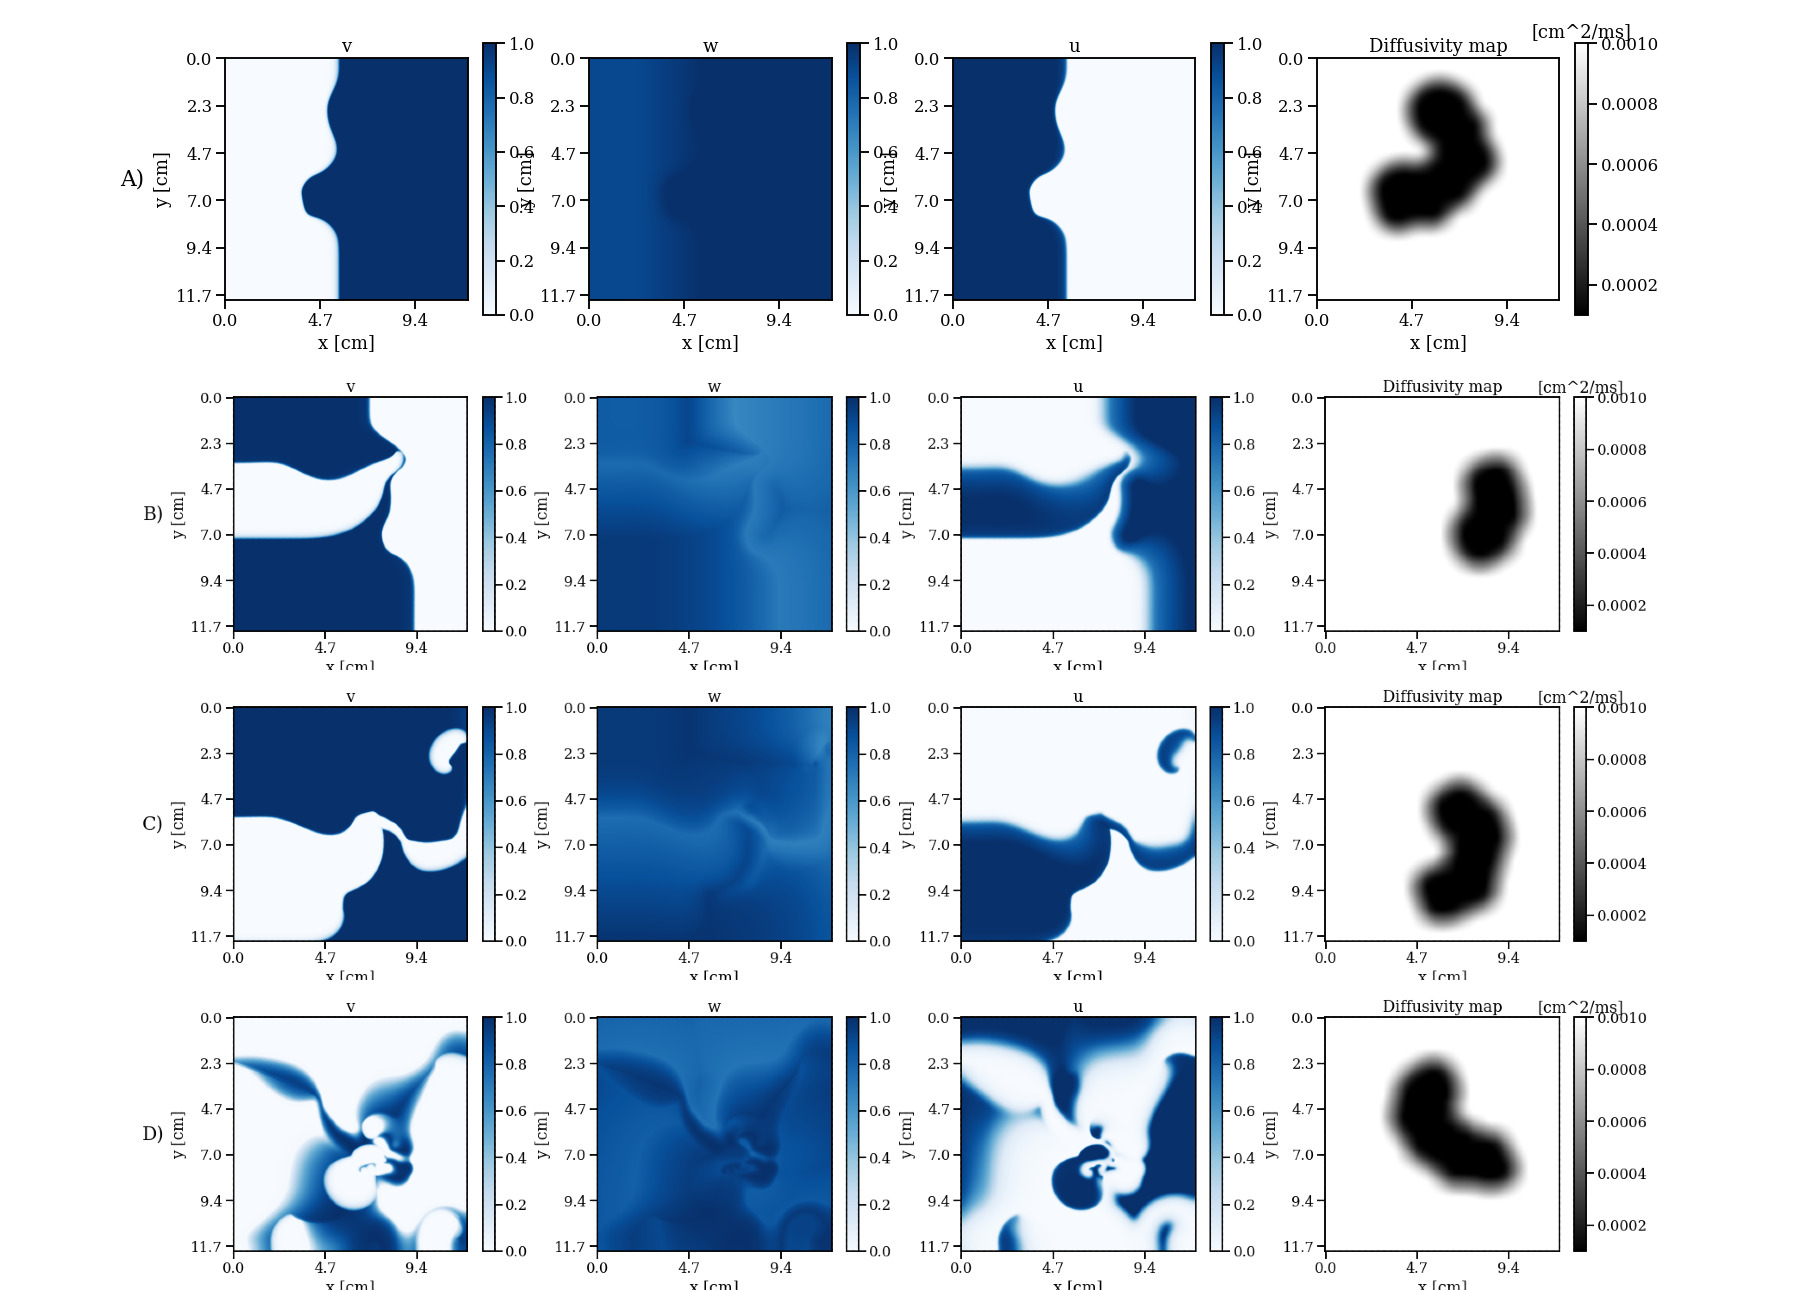
\includegraphics[width=\textwidth]{Figure-1.jpg}    
    \caption{An extract of the \textit{FKset} described in Section~\ref{sec:methods:data_generation}, showing, in each column, the three state variables, respectively, $v$, $w$, and $u$, in four different regimes (rows A-D). The last column displays the isotropic diffusivity field used for each regime.
    The set of physical parameters is the set 3 from \cite{Fenton2002}.
    Each row displays a snapshot from a different temporal sequence.
    From the top: A) a linear wave; B) the rupture of sinusoidal rhythm induced by the reentrant activity of a spiral wave; C) the initial phase of self-sufficient spiral, leading to a potential arrhythmia; D) fibrillation induced by disorganised re-polarisation resulting in a pseudo-chaotic regime.
    % The results are achieved using the \textit{CardiAX} solver described in Section \ref{ch:methods}, with  $dt=0.01ms$, $dx=0.01cm$.
    Note how different diffusivity maps affect the propagation of action potential. In the presence of a low diffusivity region, the wavefront of a linear wave bends due to lower speed allowed by the tissue (row A). When the activity acquires a spiral pattern the low diffusivity region hosts the centre of the spiral (row B). The centres of the spiral waves can move within the tissue, ie. meander, as shown in row C, and also break up (row D).}
    \label{fig:1}
\end{figure}


\subsection{Problem formulation}
\label{sec:methods:formulation}
In this study, we limit the treatment of the propagation of the electrical potential to two-dimensional rectangular regions, although this formalism can be easily extended to other domains.
 
Let $X$ be a set, and $z$ a variable that ranges over $X$.
Consider the iterated function $g^k: X  \rightarrow X$ that maps the discretised state of the variable $z$ at an initial time $0$ to a future time $T$, defined as
\begin{align}\label{eq:u}
    \mathbf{z}_{T} = g^{k}(\mathbf{z}_{0}), \quad \forall k \in \mathbb{N}
\end{align}
and its related explicit Euler discretisation:
\begin{equation}\label{eq:g}
    g(\mathbf{z}_{t}) = f(\mathbf{z}_{t})\Delta t + \mathbf{z}_{t}
\end{equation}
$g^k(\cdot)$ is the Bürmann and Herschel notation for the $k$-th iterate of the function $g$, obtained by composing the function $g$ with itself $k$ times. The mapping $f: X \rightarrow X$ approximates the partial derivative of $g$ with respect to time. The Euler step size parameter is denoted by $\Delta t = T/k$.
Different discretisation techniques, such as finite difference, finite element, or spectral methods, define different representations for $f(\cdot)$.
%
We treat the problem as fully observable, using all the three variables of the Fenton-Karma equations as target values for the learning task.
By using the full state, the problem of predicting the future behaviour of the dynamical system from a known state is Markovian and can be solved without the need of a belief state that accounts for unobserved dynamics.
Further, we treat the problem also as deterministic, such that it does not require probabilistic evaluations about the next states.

\subsection{Recurrent residual neural networks}
\label{sec:methods:rnn}
To cast this discretisation scheme as a learning task, we represent the mapping $f(\cdot)$ with a neural network $f(\theta, \cdot)$, parameterised by $\theta$, and compose it recursively following $g$. We refer to the optimised model as \textit{DeepX}.
The architecture we consider is a deep residual network \cite[]{He2016DeepRecognition} composed by stacking three-dimensional convolution blocks $f: \mathbb{R}^{C \times D \times W \times H} \rightarrow \mathbb{R}^{C \times D \times W \times H}$ that preserve the initial dimension. Here $C$ denotes the set of three Fenton-Karma variables, $u$, $v$ and $w$. $D$ is the number of input states, $W$ and $H$ the width and height of the two-dimensional discretisation grid, respectively.
To describe the network mathematically we use the same notation of recursive compositionality:
\begin{align}
    r(\theta_l, (\mathbf{z}_{t})_l) &= \sigma_l(T_l (\mathbf{z}_{t})_l + B_l) + (\mathbf{z}_{t})_l \\
    h(\theta, \mathbf{z}_t) &= r^d(\theta, \mathbf{z}_t) + \mathbf{z}_t,  \quad \forall d \in \mathbb{N} \label{eq:resnet}
\end{align}
Here, the iterand $(\mathbf{z}_t)_l$ denotes the solution at layer $l$; $T_l$ is the Toeplitz matrix associated to the $l$-th convolution; $B_l$ is a bias term; $\theta_l$ is therefore the concatenation of parameters $T_l$ and $B_l$; $\sigma_l$ is a pointwise non-linear function, and $d$ is the number of function iterations, equivalent to the depth of the ResNet.
Substituting equation \eqref{eq:resnet} into \eqref{eq:u} one gets the parametric discretisation:
\begin{equation}
    \mathbf{z}_{T} = (r^d)^k(\theta, \mathbf{z}_0),  \quad \forall d,k \in \mathbb{N}
    \label{eq:odeint}
\end{equation}
where, analogously, the notation $(r^d)^k$ denotes the composition of $r$, $d$ times, then $k$ times.

We aim to find the set of parameters $\theta^*$ that minimises the expected difference $\mathcal{L}: \mathbb{R}^{C \times D \times W \times H} \rightarrow \mathbb{R}$ between the network predictions for $z_{T}$ and the solutions of the function to approximate, described below in section \ref{sec:methods:data_generation}. To formalise $\mathcal{L}$, we use the root mean squared error:
\begin{equation}\label{eq:loss}
    \mathcal{L}(\theta, \mathbf{z}_0) =
    \mathop{\mathbb{E}}_{z \in X}
    \left[
    \lVert\nabla_x \mathbf{\hat{z}}_{T} - \nabla_x \mathbf{z}_{T}\rVert_F + 
    \lVert\nabla_y \mathbf{\hat{z}}_{T} - \nabla_y \mathbf{z}_{T}\rVert_F + 
    \lVert\mathbf{\hat{z}}_{T} - \mathbf{z}_{T}\rVert_F
    \right]
\end{equation}
The variable $\mathbf{\hat{z}}_{T}$ is the network inference, $\mathbf{z}_{T}$ its associated target value. The quantities $\nabla_x$ and $\nabla_y$ represent, respectively, the spatial gradients along the $x$ and the $y$ directions, which parameterise the two-dimensional grid where the problem is defined. 
\cite{kim2019deep} and \cite{Lino2020SimulatingNetworks} reported evidence that minimising the discrepancies in the spatial gradients, together with the more usual root mean squared error between two images, improves the convergence rate of the network.


\subsection{Data generation}
\label{sec:methods:data_generation}
To generate the training data we developed \textit{CardiAX}. \textit{CardiAX} is a end-to-end differentiable, fast, finite difference solver, developed in JAX \cite[]{jax2018github}, that uses, for spatial derivatives $3^{th}$ order accuracy for the boundary points and $4^{th}$ order accuracy for the inner points, and integrates in time using the forward Euler scheme.
%
We use \textit{CardiAX} to solve the discretised version of the two-dimensional Fenton-Karma monodomain equation. The resulting time series represent the target data for the \textit{DeepX} network.
%
The data is grouped into a public dataset, which we refer to as \textit{FKset}. It is generated using explicit Euler integration scheme with a time-step of $dt=0.01ms$ and a grid spacing of $dx=0.01cm$. We experimented with different time integration schemes, namely, explicit Euler, Heun, $4^{th}$ order explicit Runge-Kutta, and Dormand-Prince. However, when compared to the forward Euler method, no detectable improvement in convergence or stability was observed by using the other time integration schemes, both in simpler and in pseudo-chaotic regimes.
In designing the dataset, we focus on a square region of insulated tissue, $12cm$ per side, resulting in a spatial grid of $1200 \times 1200$, for the finite difference model.
Data is rescaled to grids of size $256 \times 256$, corresponding to a $dx = \frac{12 \text{cm}}{ 256} \equiv 0.046875$ cm, to allow the simulations fit in the GPU memory.
\textit{CardiAX} assumes zero flow of current across the boundaries. This yields Neumann boundary conditions $\partial \mathbf{z}(\mathbf{x},t)/ \partial \mathbf{n} = 0, \forall \mathbf{x} \in \boldsymbol{\partial}\Omega $, where $ \mathbf{n}$ is the normal of the boundary $\boldsymbol{\partial}\Omega$. The parameters of the tissue used in all simulations is the parameter set 3 in \cite{Fenton2002}.

\textit{FKset} contains 120 sequences, 1000ms long, sampled at 1ms intervals. We use 100 sequences for training and 20 sequences for validation and testing.
The tissue is stimulated at the regular pace of 400 ms with spatially randomised patterns, chosen between linear waves and point stimulations.
%
Each sequence contains a unique diffusivity map to represent the presence of fibrotic tissue, which is modelled as a region of low diffusivity. This diffusivity map is generated by composing multiple overlapping irregular polygons (between 3 and 6). The border of the resulting composite polygon is then tapered using a convolution with a Gaussian filter. The position of the whole patch of fibrotic tissue is uniformly sampled within the inner portion of the domain. That is, we constrain the sampling so that the fibrotic tissue does not extend past the limits of the domain.
The resulting map $\boldsymbol{\sigma}$ ranges values between $10^{-4}cm^2/ms, 10^{-3}cm^2/ms$, representing two extremes of diffusivity for, respectively, healthy and fibrotic tissue. The upper bound is the most commonly used value in the literature, assuming a surface to volume ratio of $5000 cm^{-1}$, and a cell radius around $4 \mu m$ \cite[]{Fenton2002}. The lower bound is set to reduce the diffusion velocity just before generating a complete block of activity, which would lead to floating point underflow.

% \subsection{Evaluation}\label{ch:eval}
% The network with the lowest test error was selected as our final model. 
% Its performance was evaluated both qualitatively and quantitatively, using various test sequences, each with an unseen diffusivity map.
% Crucially, we test the limits of the model to generalise to rollouts longer than those used for training. 
% Specifically, we unroll the model for 100 re-feeds, accounting for a total of $100 \times 5ms = 500ms$ and $100 \times 5ms / 0.01ms = 5 \times 10^4$ Euler steps of the \textit{CardiAX} solver.
% Thus, the challenges these tests provide are two-fold: the generalisation to diffusivity maps never seen during training, and the high number of input refeeds, which is 50 times the one used for training, and 50000 times the ones used in the finite difference solver.

% The test sequences are constructed so that they include three different regimes: a linear wave propagating forward, a scroll wave, and pseudo-chaotic regimes. 
% From these, we take a random sample of 100 example sequences, and evaluate the differences between the simulated and predicted variables $u$, $v$ and $w$. 
% The differences between the sequences are evaluated by computing the Root Mean Squared Error (RMSE) at each time step. 
% We also show example predictions by sampling from test sequences at the time of highest error. 
% Finally, we compute the error between predictions and simulations under homogeneous diffusivity conditions, to further test the prediction capability of the model. 

\subsection{Algorithm}
\label{sec:algorithm}
The development of \textit{DeepX} follows the paradigm of supervised learning with stochastic gradient descent (SGD). We aim to fit a parametric function to an empirical data distribution by: uniformly sampling from it; evaluating the distance to the target value; calculating the gradient of the loss with respect to the parameters and, finally, updating them using a form of stochastic gradient descent.
We refer to a \emph{state} of the system $s(t)$ as the concatenation of the three Fenton-Karma variables at an instant of time $t$: $\langle u(t), v(t), w(t)\rangle$, and to a \emph{simulation} as a sequence of states $\{s_i \, | \, t < i < T \in \mathbb{N}\}$.
The optimised function $f(\theta^*, \cdot)$ maps a state of the system $s(t)$ to the next state $s(t+1)$.
Inference for longer sequences is performed as described in equation \eqref{eq:odeint}. The last function evaluation is recursively re-used as an input for the calculation of the next state.

The core of \textit{DeepX} is a Convolutional Neural Network (CNN). CNNs learn a set of small kernels, $3 \times 3 \times 3$ in this case, used to convolve the input field at each layer.
An interesting property of this operation is that it is agnostic to the size of the input. By increasing the number of iterations in the dimensions of the convolution (e.g. rows and columns), the CNN accommodates for different input sizes. This operation is invariant to translations.
For details on the model architecture and the optimisation procedure see the supplementary material, section \ref{sec:supp:architecture} and \ref{sec:supp:optimisation}.

To monitor overfitting during the optimisation procedure, we sample from a held-out validation dataset not used for training, performing 5-step rollouts.
To test the model on more realistic scenarios we use data and parameters outside the distribution used to optimise the model, thus considered out of distribution (OOD). In particular, tests are performed on the same validation dataset but using 20-steps rollouts. 
%        

\begin{figure}[tb]
    \centering
    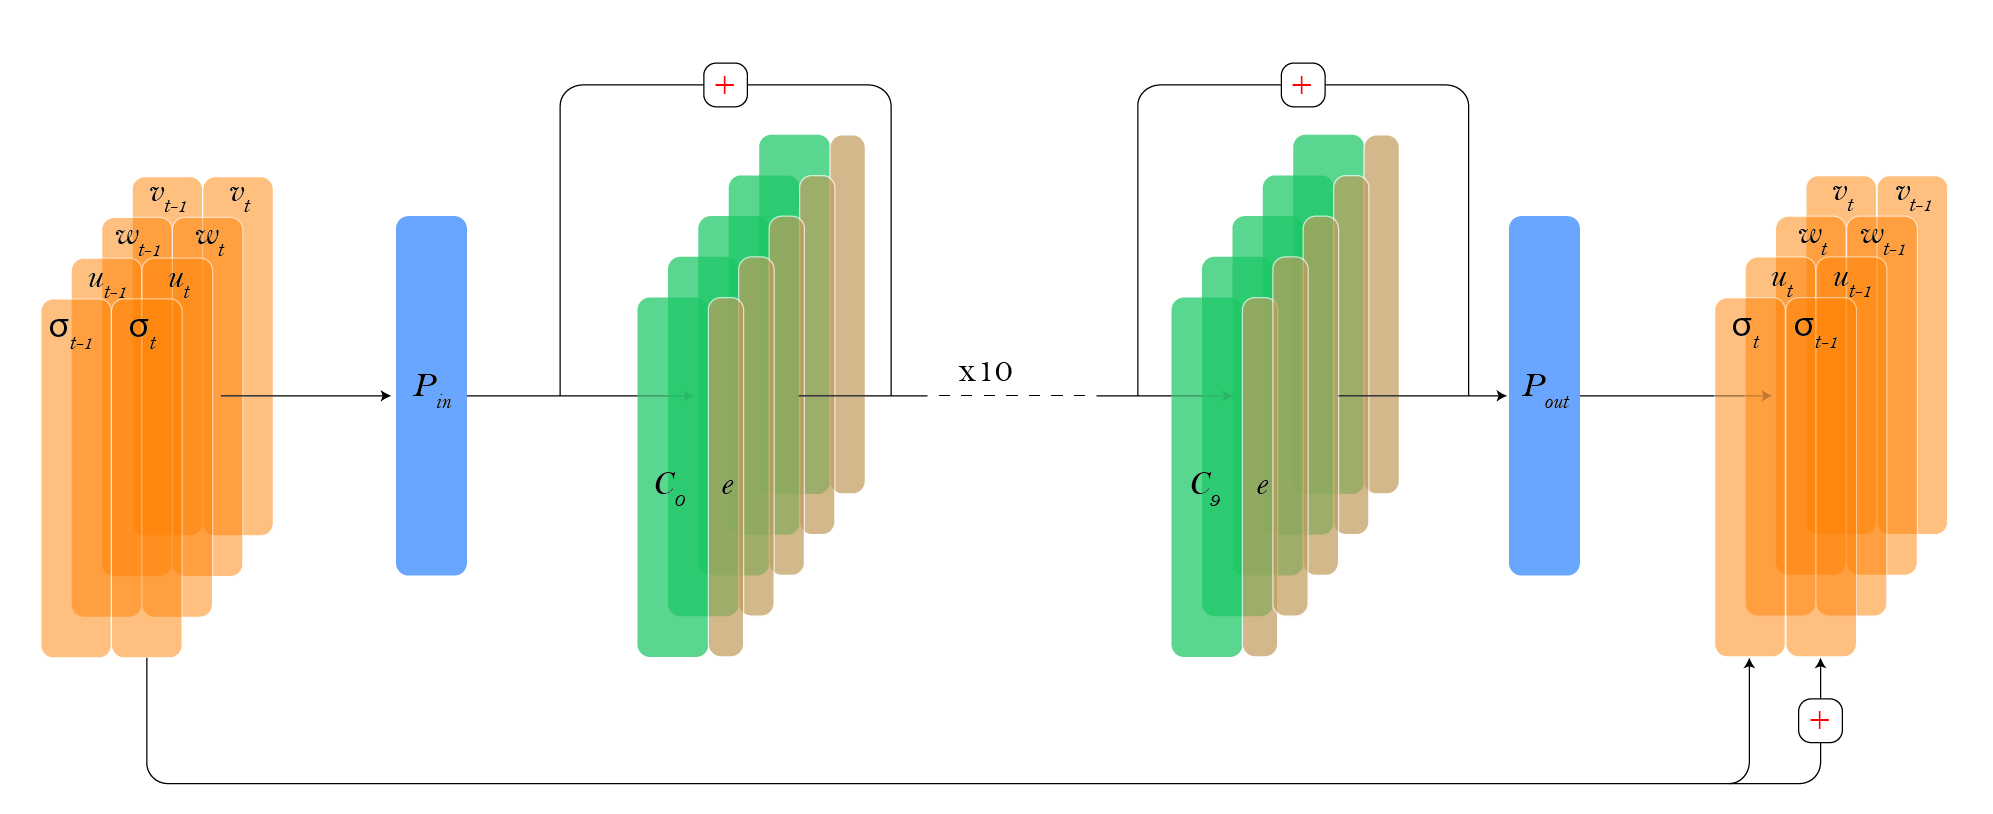
\includegraphics[width=\textwidth]{Figure-2.jpg}
    \caption{
    Architecture of the proposed residual convolutional network, where: $\boldsymbol{\sigma]}_t$ is the diffusivity map at time $t$; $u_t$, $v_t$ and $w_t$ are the three Fenton-Karma variables at time $t$; $P_{in}$ is the preprocessing function; $C_l$ is the convolution at layer $l$, and $e$ is the exponential linear unit (ELU) function.  There are 10 convolutional layers in the architecture, each with its own set of filters. $P_{out}$ is the posprocessing function, compressing the latent convolution dimension into the three Fenton-Karma variables. Plus signs between convolutions indicate residual connections, whilst the last addition represents the forward Euler scheme. 
    }
    \label{fig:network}
\end{figure}



\subsection{Evaluation metrics and chaoticity}
\label{sec:methods:evaluation}
The Root Mean Squared Error (RMSE), or Frobenius norm, is cornerstone to evaluate model performance in deep learning, and the most widely used metric to statistically compare static spatial fields.
Small RMSE values often signify that the trained model faithfully reproduces the mapping of input-output pairs in the experimental data.
% Chaoticity 
However, models of cardiac electrophysiology often present chaotic or multi-periodic dynamics.
\cite{lombardo2019chaotic} showed that the presence of heterogeneities is sufficient to generate spiral waves whose tip present chaotic dynamics.
\cite{sohn2019scale} presented evidence that Lagrangian coherent structures, special surfaces of action potential trajectories with the power to organise the rest of the flow, are non-stationary in the Fenton-Karma ionic model, despite invariant to scale.
At the cellular scale, \cite{dai2010chaos} studied the chaoticity of the solution to the Echebarria–Karma modulation equation \cite[]{echebarria2002instability} for action potential duration alternans in a cardiac fibre.
In summary, the two-dimensional monodomain equation coupled with the Fenton-Karma ionic model shows inherently chaotic dynamics.

% RMSE in chaos
Under these conditions, that is when dealing with spatio-temporal data and dynamical systems that show chaotic behaviour, small localised errors can be amplified over time. The recurrent nature of the model, and the non-stationarity of the error induced by the discretisation of a continuous model, are its main causes.
This happens regardless of the discretisation method. For example, finite difference and spectral or finite element models can converge to different orbits for the same initial conditions, due to chaotic or multi-periodic dynamics \cite[]{skardal2014coexisting}.
The RMSE norm focuses on localised (point-wise) discrepancies, which can be a useful error signal to train the network, but fails to capture higher level dynamical features, such as the temporal consistency between two consecutive instants belonging to the same sequence.
The RMSE’s extreme locality and the recurrent nature of the dynamical system combined causes the RMSE to increase over time. This is particularly visible in long predictions.

As our aim is not to fit chaos, the RMSE is not sufficient on its own to provide a robust measure of distance between two estimators for action potential propagation.
The inadequacy of the RMSE metric to capture higher level features of action potential propagation is also highlighted by \cite{Herzog2018}, which proposes the alternative Jensen-Shannon divergence (JSD) to assess the plausibility of predictions. 
However, the JSD does not have an immediate biological interpretation.
Therefore, to mitigate the problems of these evaluation procedures, we seek to complement the RMSE and the JSD by extracting physiologically significant features from the time series. We then evaluate the estimators, \textit{CardiAX} and \textit{DeepX}, in the space of these features.
As \cite{Fenton2002} states, these physiological quantities play a more fundamental role for modelling wave dynamics than the shape of the action potential.
The use of alternative measures of the quality of two predictions is used, for example, in anatomical image segmentation, as no single metric is optimal for different types of spatial prediction \cite{taha2015metrics}.

Finally, to investigate the robustness to different conditions, test sequences comprise two different dynamical regimes, linear and spiral waves, and two different diffusivity conditions, heterogeneous and homogeneous diffusivity map.


\subsubsection{Electrograms}
\label{sec:methods:evaluation:electrograms}
Extracellular electrical potential $\phi_{e}(V)$ is computed as described by \cite{spach1979extracellular} and \cite{varela2014role}. The methods integrates the voltage in space and time around the electrode using a Green's function kernel:
\begin{align}
\phi_{e}(V) = K \int\int{ \frac{\nabla \cdot (\boldsymbol{\sigma}\nabla V)}{\sqrt{(x-x_{e})^{2}+(y-y_{{\rm e}})^{2}}}} dx\,dy
\end{align}
Here, $\phi_{e}$ is the electric potential measured in a single electrode; $x_e$ and $y_e$ are the positions of the electrode in the finite difference grid; $\boldsymbol{\sigma}$ is a scalar field that captures the local diffusivity.
16 Electrodes are placed in a $4 \times 4$ grid, 1.5 cm away from the surface along the normal vector, with a mean inter-electrode spacing of 3 cm. $\phi_{e}$ is computed every 5 ms, the integration step of the network.

\subsubsection{Centres of rotors}
\label{sec:methods:evaluation:rotors}
A useful feature to better understand the dynamics of action potential is the identification of spiral wave tips. Rotors are tracked following the methods described in \cite{Fenton1998}. We choose an arbitrary isopotential contour $V(x, y) = \bar{V}$ that represents the frontier between depolarised and polarised regions. The intersection between two isopotential lines describes a point of constant potential, thus the tip of the rotor:
\begin{align}
    V(x, y, t) - \bar{V} = \partial V(x, y, t) = 0
\end{align}
In the experiments we set $\bar{V} = 0.7$.
Control rotors are used as a baseline to evaluate the performance of the deep learning model. Trajectories are built using a random walk procedure.
Specifically, we develop each control trajectory in time by randomly generating the direction and the magnitude of the displacement at each time step. The former is drawn as one of four possible directions (positive or negative in both the x and the y direction, or positive in one direction and negative in the other). The displacement magnitude is drawn from an empirical distribution obtained from the original trajectories. All control trajectory for a given sample simulation start from the same spatial coordinates as the corresponding \textit{DeepX} rotor trajectory..

\subsubsection{Action potential dynamics}
\label{sec:methods:evaluation:maps}
Finally, we compute a series of time activation maps that play a fundamental role in determining the properties of waves in excitable media.
The Action Potential Duration (APD) map described the time interval necessary for the membrane to partially recover its resting properties. We set the threshold at 90\% the repolarisation of $u$m the \textit{APD~90}. The importance of the APD has been emphasised by numerous study \cite[]{boyett1978study, elharrar1983cycle}, for its capacity to incorporate a relevant proportion of the ionic dynamics.
% %
The Conduction Velocity (CV) restitution map measures the maximal velocity of an excited wavefront moving through the myocardium. The CV is the direct complement of the APD as it described the properties of the tissue as it returns to its resting state. CV maps are computed using the formalism described in \cite{cantwell2015techniques}.
These two quantities regulate the dynamics of, respectively, depolarisation of the wavefront and repolarisation of the waveback, playing a fundamental role in modelling action potential dynamics \cite[]{Fenton1998}.
% %
The Resting Membrane Potential (RMP) is the difference of action potential between the cellular membrane and its surroundings when the cell is not excited.
RMP is computed as the minimum of the action potential over time, for each point in space: $\min_{t} (u_t(x))$, as described in \cite{varela2016atrial}.
% %
Activation Times (ATs) are calculated by finding the time that corresponds to the maximal change of action potential after each excitation.
% %
The Action Potential Amplitude (APA) is computed as the difference between the action potential the time before and after the arrival time. Note that in our experiments it is likely to be underestimated due to discretisation.
% %
For the detailed formalism on how to calculate RMP, AT and APA we referred to \cite{varela2016atrial}.

In the following chapters, we refer to this set of measures as \textit{activation maps} or simply \textit{maps}.

\section{Results}
\label{sec:results}
In the following experiments we apply the evaluation procedure described in \ref{sec:methods:evaluation} to investigate the performance of our model. Were not specified, the simulations used for the analyses are performed by solving the Fenton-Karma monodomain equation on both homogeneous and heterogeneous media and can present rotational dynamics with their break up following fibrillation. 
The exact architecture used to generate \textit{DeepX} sequences is described in \ref{sec:supp:architecture}, and its relative optimisation procedure in \ref{sec:supp:optimisation}.
The first section presents the results using canonical evaluation metrics and shows the problems of using those to evaluate the models.
The next sections compare the solutions of \textit{DeepX} against the \textit{CardiAX} simulations using electrophysiological measures chosen because of their relevance from a clinical and biological perspective. As described in section \ref{sec:methods:evaluation}, we use the following: a) electrograms predictions, b) dynamical behaviour of rotors, c) action potential dynamics.
Finally, we conclude by showing the results on tissue sizes different from the ones used during training.
Every data used in these experiments has not been used for training.

\subsection{Inference}
\label{sec:results:inference}
Here, we evaluate \textit{DeepX} under the canonical evaluation metrics discussed in \ref{sec:methods:evaluation}, RMSE and JSD, to allow comparison with the wider literature and to contextualise the performance of our model.

% conditions
Figure~\ref{fig:3} shows the evolution of the errors over time on 40 randomly sampled simulations, 10 for each condition: heterogeneous and homogeneous tissue with either linear or spiral waves. For each condition we plot the errors against a baseline represented by a constant field of 0.5. The baselines sets an upper bound for both the RMSE and the JSD.
%  spiral waves
We observe that in the case of spiral waves ($a$ and $c$ in figure~\ref{fig:3}) the error is low at the beginning of the simulation, and then consistently grows with time, despite not strictly monotonically.
% linear waves
Instead, the simulations containing only linear waves ($c$ and $d$ in figure~\ref{fig:3}), show a different evolution. The error grows in the first part of the simulation, then decreases with time. 
% generalisation to homogeneous tissue
On the orthogonal dimension of type of tissue, we observe that the errors are, in the pairs of wave types, very close between the homogeneous and heterogeneous case.
% performance with small training window
The vertical grey line in figure~\ref{fig:3} represents the horizon of the integration used in training. That is, the network has been optimised to predict the next 5 frames (each distant $5$ms from the precedent, for a total of $25$ms) as close as possible to the \textit{CardiAX} simulations. 
By unrolling the network up to $200$ times ($10^2$ more), we can simulate sequences up to $1$s, for which the training frontier represent just a small fraction of time.

Figure~\ref{fig:4} shows the correlation between the RNMSE and the JSD, extracted from the same data. The two errors are equally informative in the case of linear waves, and in turn in non-chaotic scenarios.
Instead, the correlation breaks in the case of spiral waves, especially in the middle of a simulations, where time is represented using colours.

In figure~\ref{fig:5}, we decompose the error to identify which part of the ionic model contributes to the highest error.
Most of the error in the case of linear wave is contained into the action potential alone. On the contrary, when spiral waves and wave break-ups start to appear, the $v$ variable, responsible for gating the activity of the $u$ variable shows similar level of errors. 
The $w$ variable, which balances $u$ during the resting phase, shows small errors overall.
% 
One interesting phenomenon that we observe in the simulations produced by \textit{DeepX} is high frequency oscillations in the errors.
This is particularly evident when the tissue is in recovery. In figure~\ref{fig:3} we can observe that, in the case of linear waves, when the RMSE decreases, and the tissue settles back into the resting potential, the JSD starts to oscillate at this high frequencies.
This inaccuracy of the model when the tissue depolarises is congruous with the results on the resting membrane potential, later discussed in \ref{sec:results:maps}.
One hypothesis that can explain this symptom is the high variance of spatial gradients between the $w$ variable and the $u$ and $v$ variables. This difference could require the neural network to learn a very diverse set of convolutional filters to approximate such variance, making the optimisation problem more difficult.


\begin{figure}[!htp]
\centering
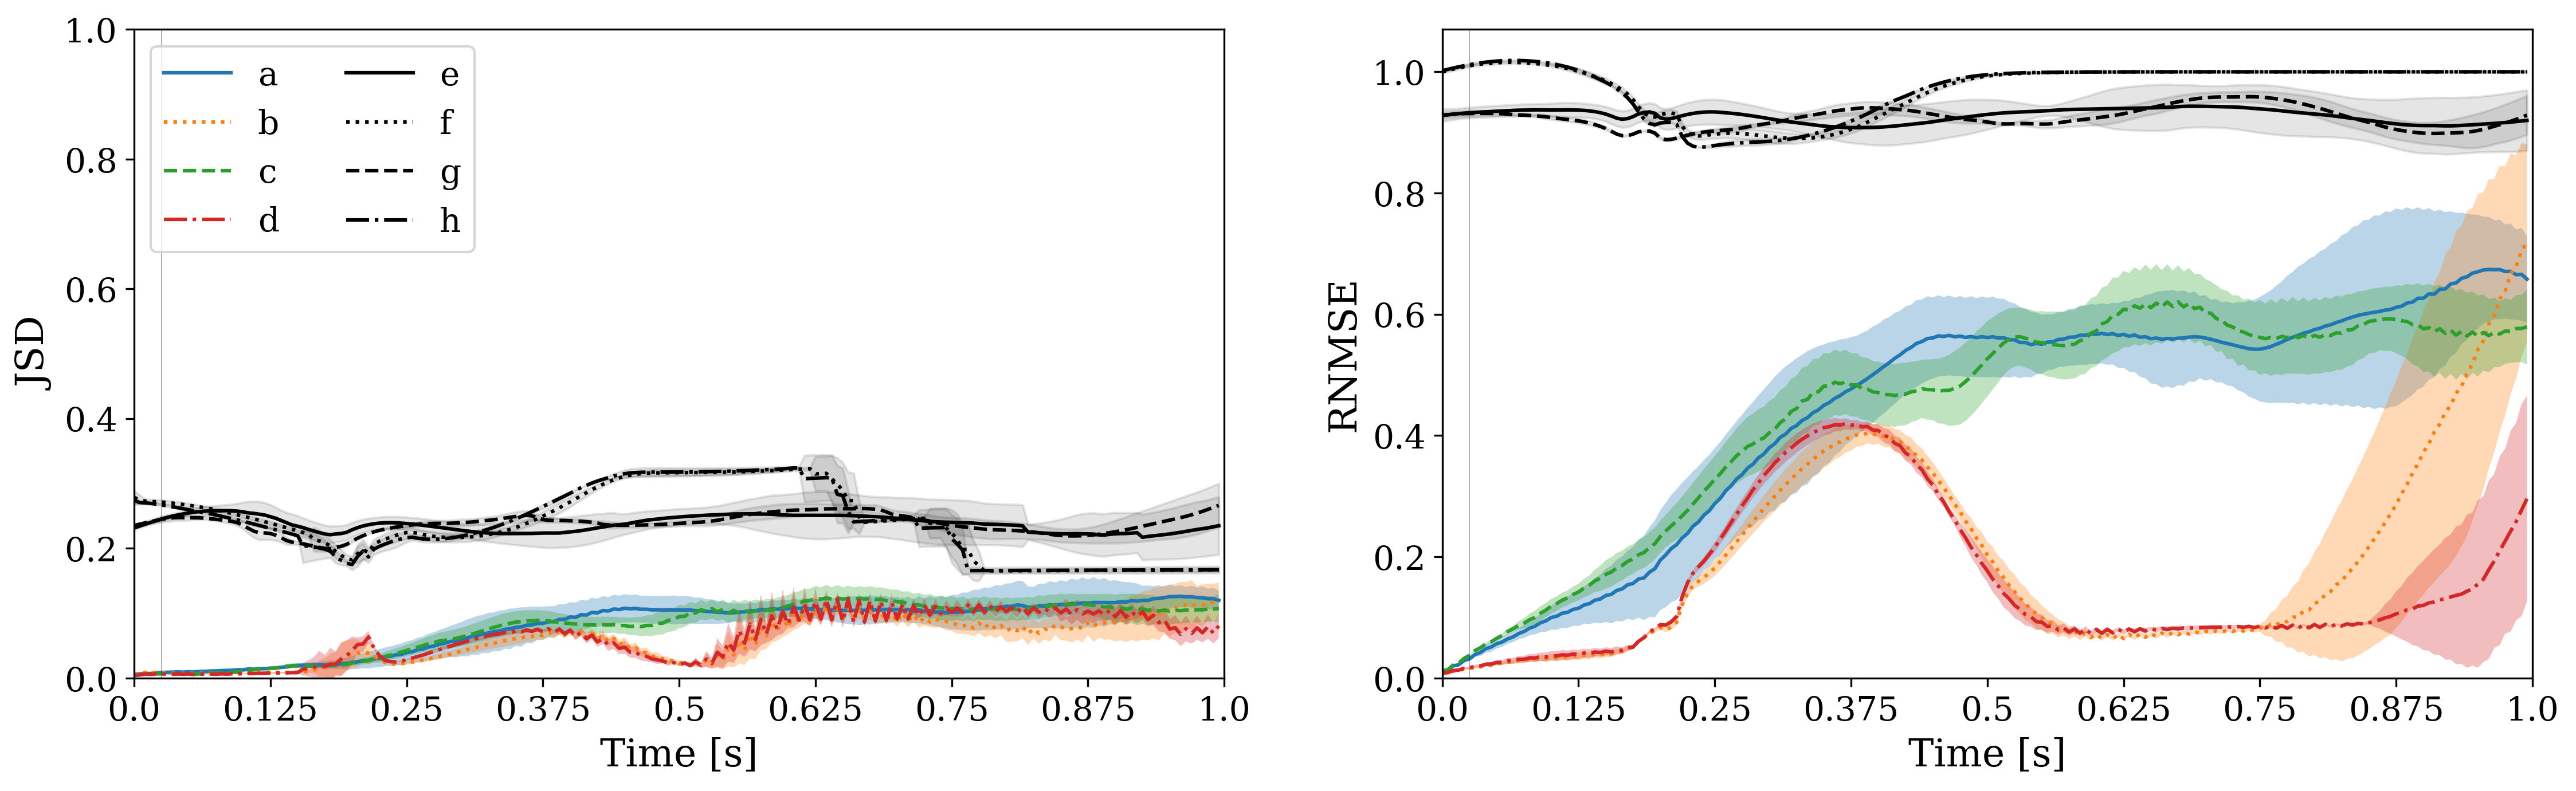
\includegraphics[width=\textwidth]{Figure-3.png}
\caption{JDS and RNMSE between \textit{CardiAX} and \textit{DeepX} simulations. Each line shows the mean over 10 runs and the spread area represents their standard deviation. a) Spiral wave in heterogeneous tissue; b) linear wave in heterogeneous tissue; c) spiral wave in homogeneous tissue; d) linear wave in homogeneous tissue. e), f), g) and h) are the respective baselines, obtained by applying the metric between the \textit{CardiAX} simulation and a constant field at 0.5. The thin vertical grey line shows the temporal horizon used for training.
}
\label{fig:3}
\end{figure}

\begin{figure}[!htp]
\centering
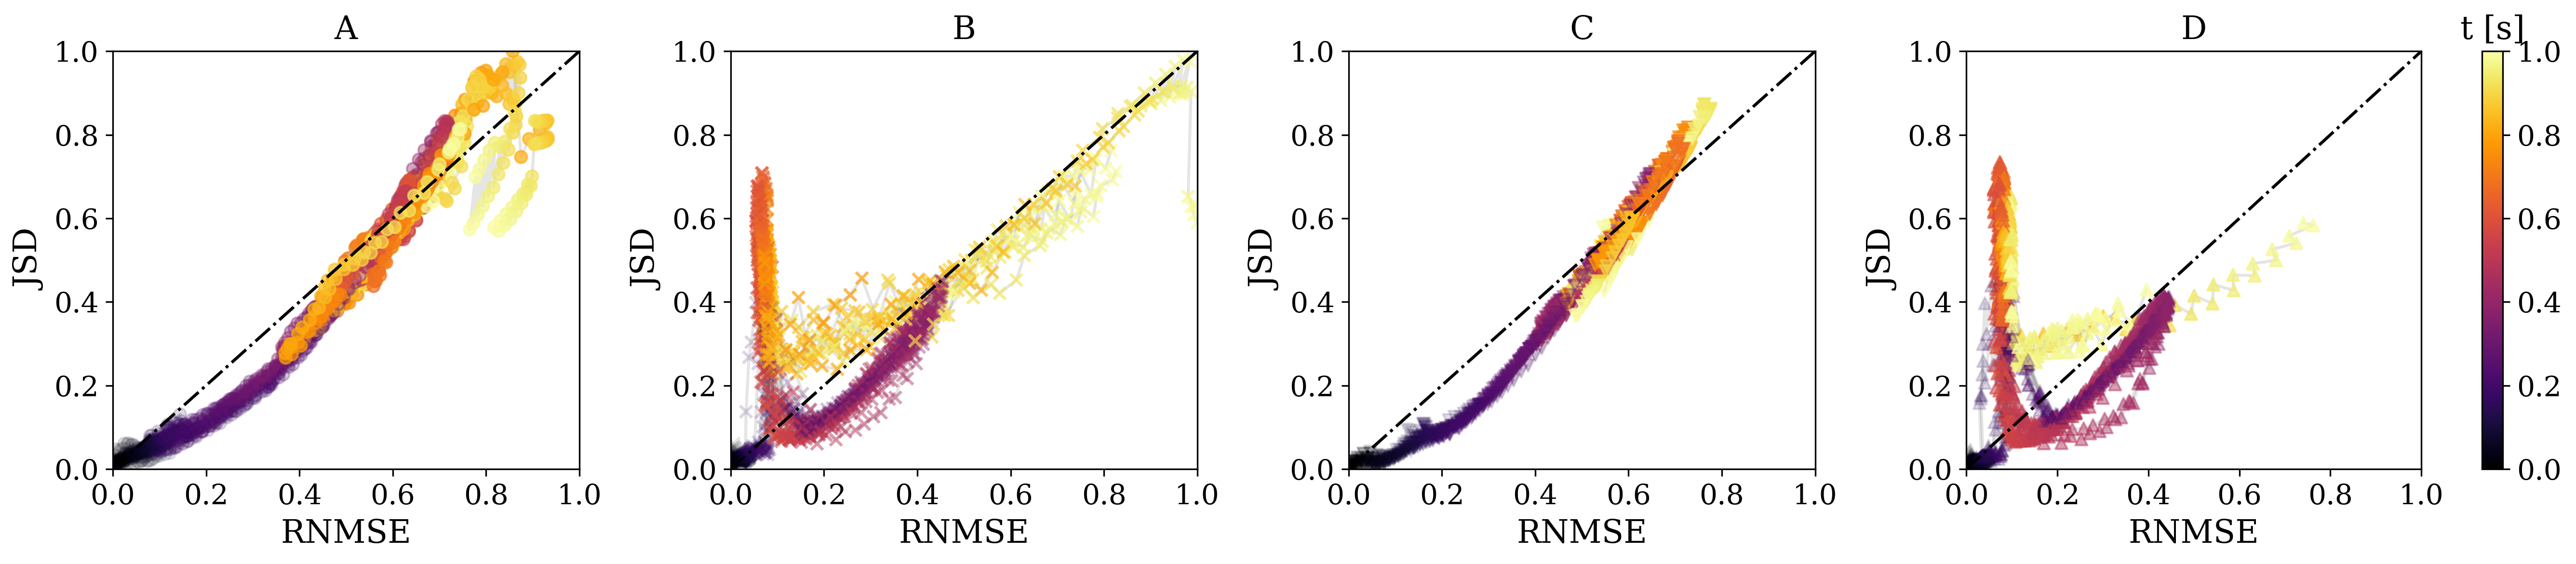
\includegraphics[width=\textwidth]{Figure-4.png}
\caption{Correlation between the JSD and RNMSE metric between \textit{DeepX} and \textit{CardiAX} simulations. For each plot, both metrics have been min-max normalised in the range $[0, 1]$. A) Spiral waves in heterogeneous tissue, B) Linear wave in heterogeneous tissue, C) spiral waves in homogeneous tissue, D) Linear wave in homogeneous tissue. Each plot shows the analysis for 10 randomly sampled simulations. Colours represent time in seconds, and grey lines connect individual temporal sequences. The black lines set perfect correlation.
}
\label{fig:4}
\end{figure}


\begin{figure}[!htp]
\centering
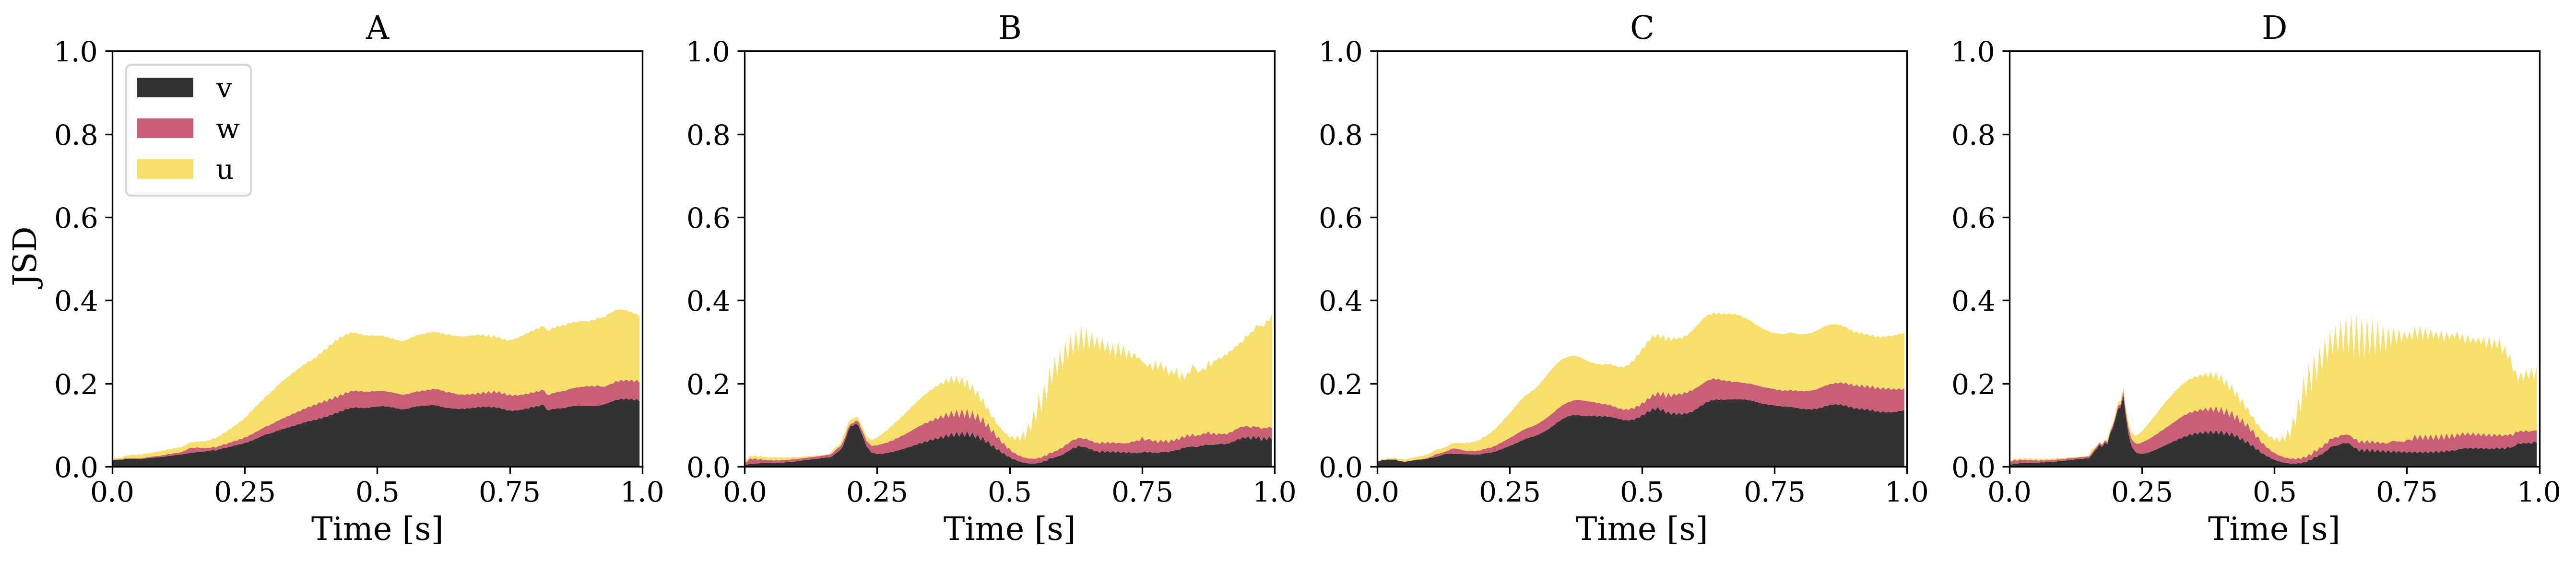
\includegraphics[width=\textwidth]{Figure-5.png}
\caption{Stacked area chart of the decomposition of the JSD in each variable of the Fenton-Karma model. The error for each variable is displayed on top of each other. A) Spiral waves in heterogeneous tissue, B) Linear wave in heterogeneous tissue, C) spiral waves in homogeneous tissue, D) Linear wave in homogeneous tissue. JSD values are averaged over 10 randomly sampled run for each condition, for a total of 40 runs.
}
\label{fig:5}
\end{figure}
% As observed in many cardiac models \cite[]{Shajahan2007Spiral-waveTissue}, and confirmed by \textit{in-vivo} experiments \cite[]{Hwang2005Complex-periodicInhomogeneities}, the centre of spiral waves is likely to stabilise 


\subsection{Electrograms}
\label{sec:results:electrograms}
In this section, we refer to a pair of electrograms as two time series, derived from \textit{CardiAX} and \textit{DeepX} solutions and computed on corresponding electrodes (i.e. same ID).
To quantify the similarities between traces we compute the Pearson correlation coefficient between the two time series in each electrogram pair, that is we measure the \textit{linear} correlation between the two signals. Figure~\ref{fig:6} shows the distribution of correlation coefficients across all pairs of electrograms under four different experimental conditions: homogeneous and heteregeneous media, for both linear and spiral wave dynamics. These distributions are represented by the blue lines.

\begin{figure}[!htp]
\centering
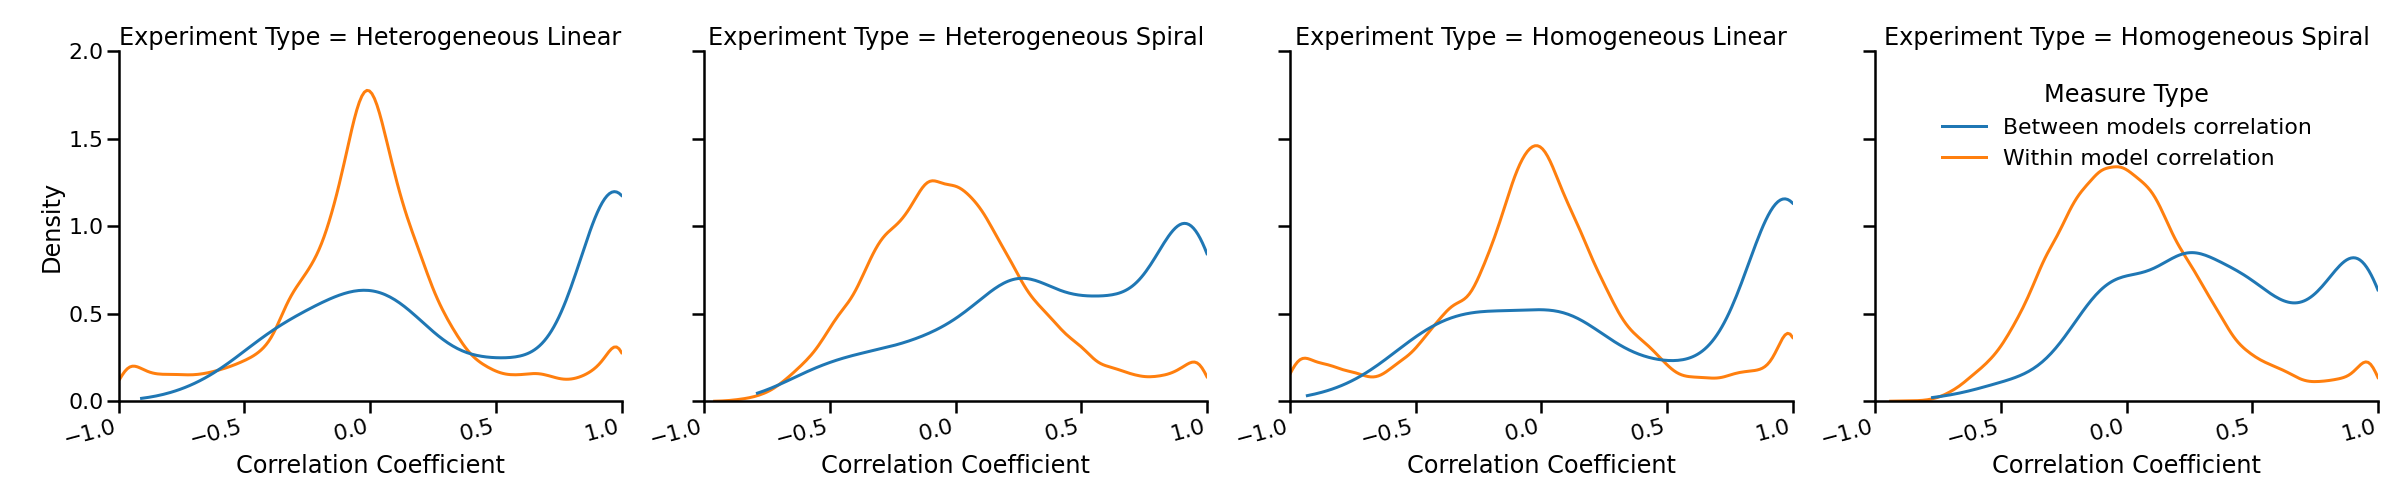
\includegraphics[width=\textwidth]{Figure-6.png}
\caption{ 
%(a) Distribution of the correlation coefficients between pairs of electrograms computed on corresponding electrodes (i.e. same ID), but from different models (``between model'' correlation coefficients).(b) 
Distributions of ``between model'' (blue lines) and ``within model'' (orange lines) correlation coefficients. These are evaluated across four different experimental conditions (homogeneous or heterogeneous diffusivity maps and linear or spiral wave dynamics). ``Between model'' correlation coefficient are those computed between pairs of electrogram traces derived from different electrodes, but from the same model. ``Within model'' correlation coefficients are those computed between two electrograms derived from the same electrode, but different models.
}
\label{fig:6}
\end{figure}

Our results show that, while the highest density is around 1, all distributions extend to negative correlation coefficients as well. The distribution average is similar across experimental conditions, ranging between $0.37$ and $0.42$. 
Some of the low or negative correlation coefficients may be explained by the time shifts (or delays) that were observed in the neural network predictions. 
% To test for this, the analyses could be extended to take into account the peak of the cross-correlation functions.

As an example of such occurrences, figure~\ref{fig:7} shows two series of 16 electrogram pairs (for a total of 32 pairs) from simulations in the case of heterogeneous diffusivity with: (a) spiral and (b) linear wave dynamics.
In most pairs, the electrograms from the deep learning model closely follow those from the finite difference model, with some of them diverging over time. 
Some of these discrepancies, however, are caused by the neural network simulations having similar, but delayed, dynamics with respect to the numerical ones (e.g. ID $2$ in Figure\ref{fig:7}a).
These delays in the signal between the \textit{CardiAX} and the \textit{DeepX} simulations could account for some of the low or negative correlation coefficients observed.

\begin{figure}[!htp]
\centering
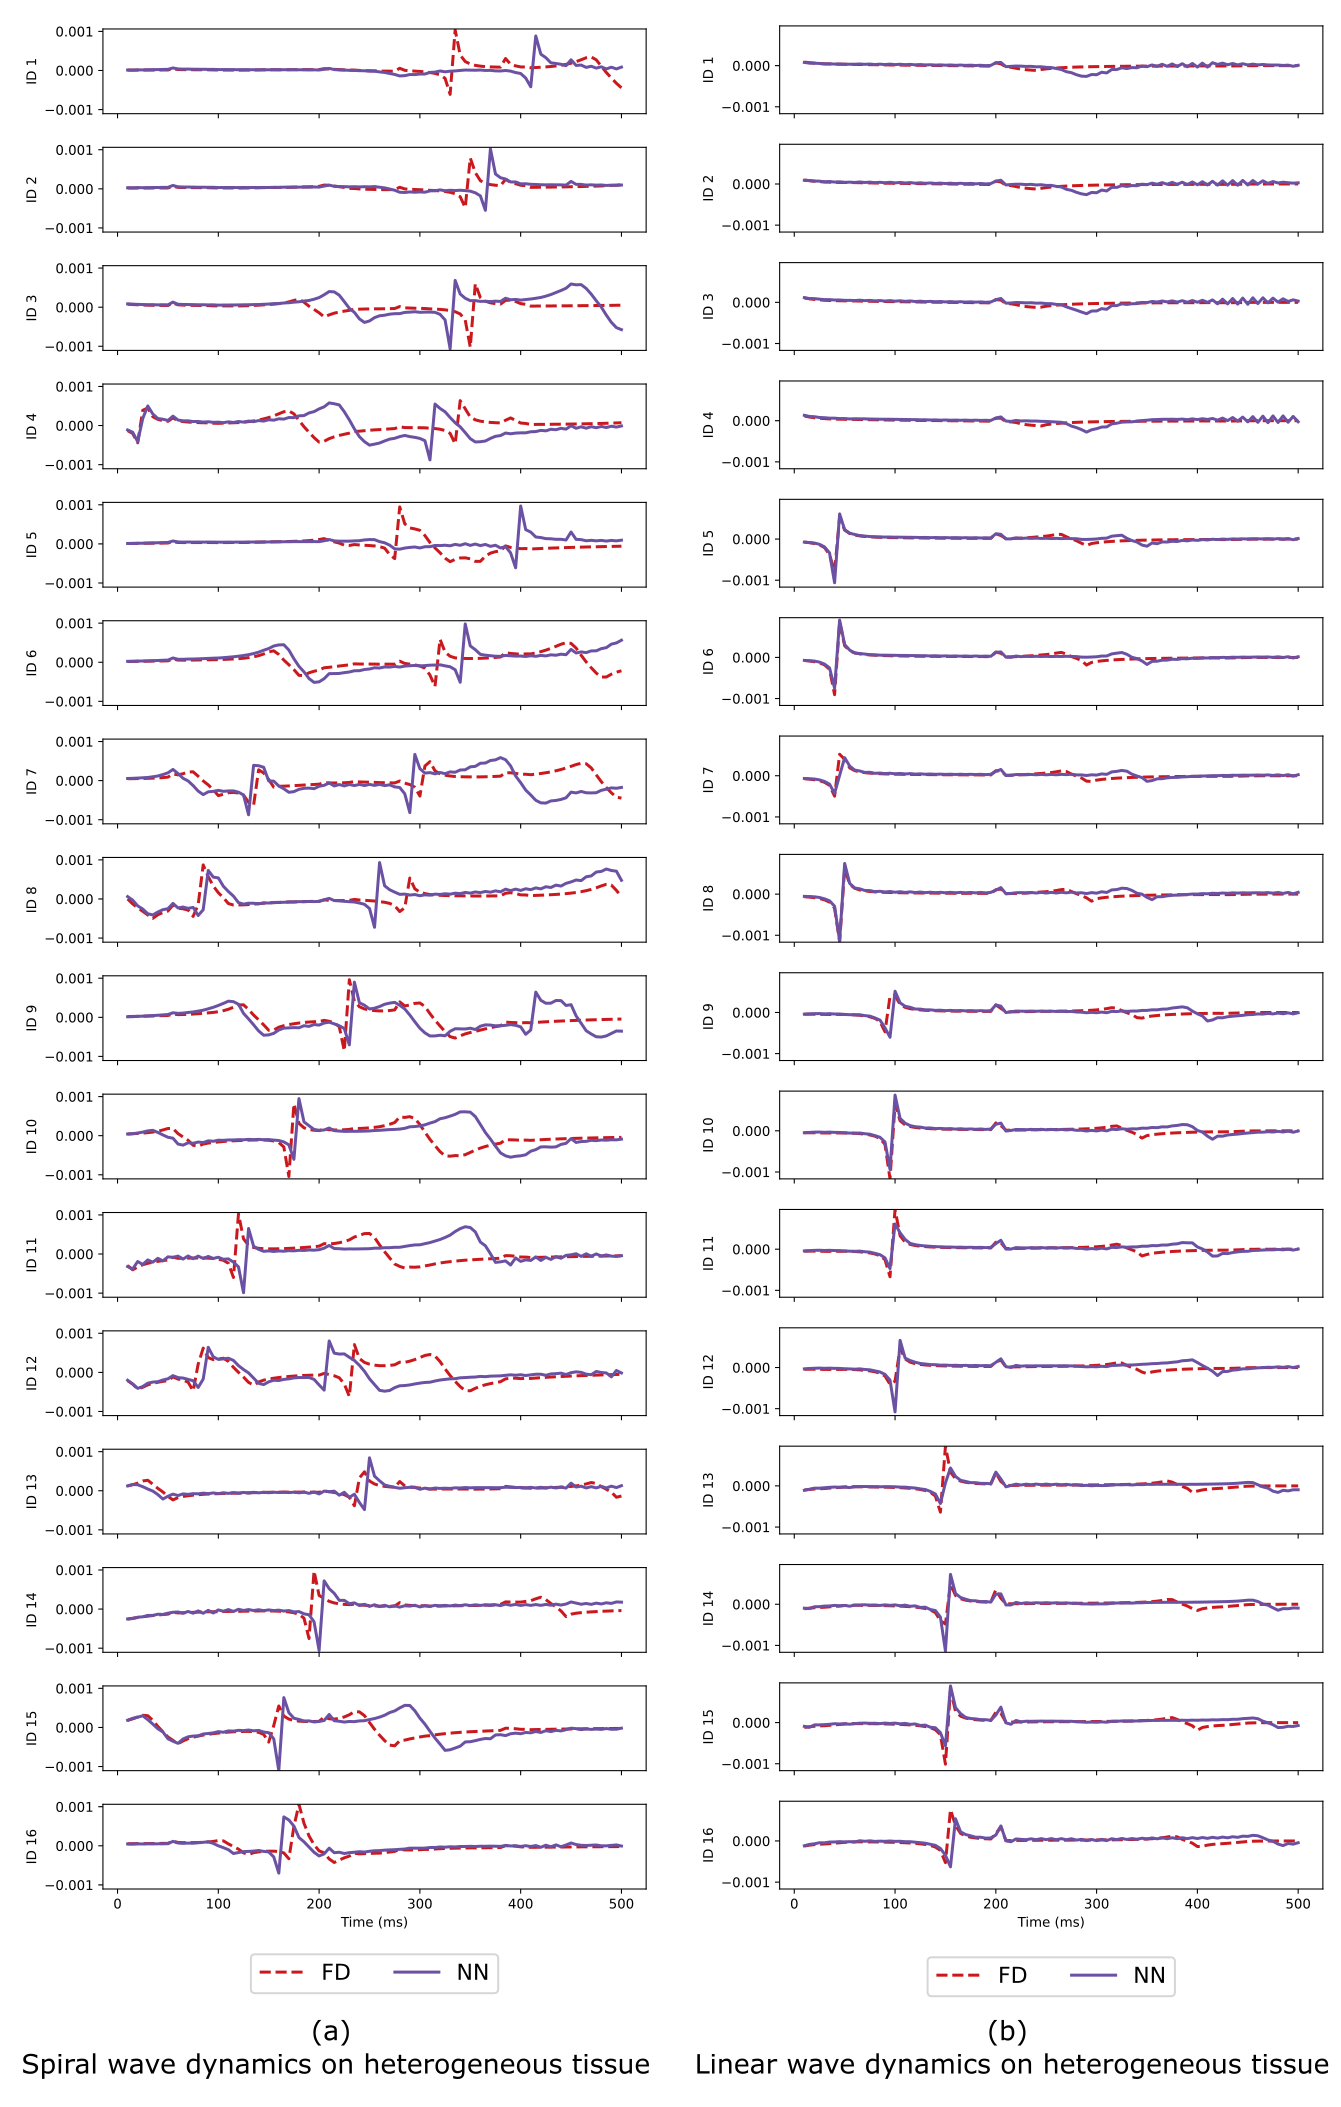
\includegraphics[width=.73\textwidth]{Figure-7.png}
\caption{A sample of electrograms computed from \textit{CardiAX} (dotted, red lines) and \textit{DeepX} (solid, purple lines) simulations in the case of heterogeneous diffusivity. On the left, (a) shows the electrogram in the case of spiral dynamics; on the right, (b) shows the case for a linear wave propagation.
}
\label{fig:7}
\end{figure}

To obtain a control measure, we compared the distribution of correlation coefficients against a baseline.
That is, we computed the correlation coefficient between pairs of electrogram traces computed on different electrodes (i.e. different IDs), but from the same model.
We refer to these as ``within model'' correlation coefficients, as opposed to the ``between model'' introduced above.
Figure~\ref{fig:6} shows the distributions of ``within model'' (orange lines) and ``between model'' (blue lines) correlation coefficient under all possible conditions. 
We observe that ``between model'' correlation coefficients tend to be higher than their ``within model'' counterpart.
%
To confirm the statistical significance of our results, we performed a series of Kolmogorov-Smirnov tests with Bonferroni correction. 
We implemented two sets of one sided tests, first to assess the null hypothesis of ``between model'' correlations being greater than ``within model'' ones, then to assess the opposite 
Resulting p-values for the former were close to $1$, and $0.001$ for the latter. These results indicate that \textit{DeepX} is able to generate predictions that result in electrogram traces that are significantly more similar to those obtained from finite difference simulations than to the baseline.

%%%% ROTORS TRACKING
\subsection{Tracking of rotor tips}
\label{sec:results:rotors}
We then assessed how well our model can track spiral rotational activity.
%
Figure~\ref{fig:8} shows two examples of rotor trajectories computed from both the \textit{CardiAX} and the \textit{DeepX} model, in the presence of spiral wave dynamics with heterogeneities.

Figure~\ref{fig:9} shows the absolute errors between the euclidean distance of two rotor trajectories from numerically simulated and predicted data, aggregated across multiple simulations\footnote{When aggregating across trajectories we interpolate all of them along a common time vector.}. Lines show the average value across 20 simulations, while shaded areas represent the standard deviation. %are the $95$\% confidence interval across all simulations.
For comparison, we also show the control distribution of errors, designed, for each simulation, as the euclidean distance over time between $100$ random walks and the \textit{CardiAX} trajectory. Section~\ref{sec:methods:evaluation:rotors} describes how these control trajectories were computed. 

\begin{figure}[!htp]
\centering
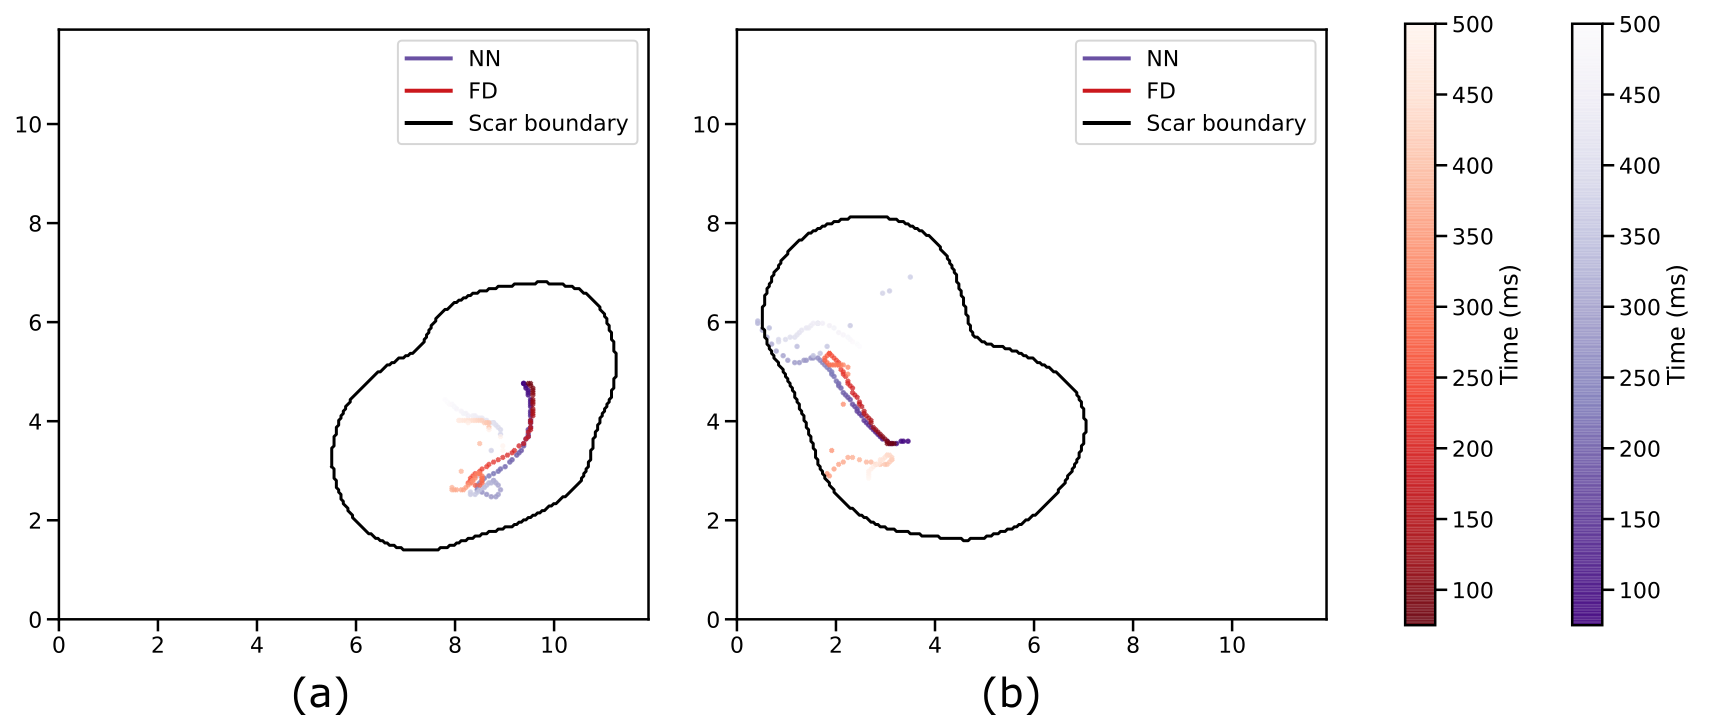
\includegraphics[width=.9\textwidth]{Figure-8.png}
\caption{Example rotor trajectories computed for both the numerical (red markers) and the machine learning (purple markers) model in the presence of spiral wave dynamics with heterogeneous diffusivity maps. Each circular marker represents the position of the rotor at a given instant in time, where time is represented by increasing lightness values of the corresponding colours.
}
\label{fig:8}
\end{figure}

The distances between the \textit{DeepX} and the \textit{CardiAX} tips are on contained under 5.4 cm for the heterogeneous case and 6.4 cm for the homogeneous one (as opposed to 14.7 cm and 20.4 cm, respectively, for random trajectories).
Thus, while the difference between numerically simulated and predicted trajectories increases over time, consistent with the assumption of chaoticity of the dynamical system, their values are bounded above by the control measures.
We also report the average difference between the time of onset of the rotors between the two models as $21.30$ms. 

In figure~\ref{fig:10}, we observe that, despite figure~\ref{fig:9} showing \textit{DeepX} and \textit{CardiAX} tips moving apart from each other, they both converge towards the boundary of the scar.
This is the same behaviour observed in section~\ref{sec:results:rotors}, that is the pinning of the spiral wave to localised inhomogeneities.
The distance is assigned a positive value when the rotor is inside the scar, and negative when it is outside.
The lines represent the average across simulations, whilst shaded areas represent the standard deviation. %$95$\% confidence interval of the mean.
This results show that all trajectories from finite difference and neural network simulations orbit around the scar boundaries, while the control trajectories do not. Instead, they tend to drift away from the fibrotic tissue at a constant rate.
Furthermore, we computed the correlation coefficient between the distance from the scar boundary over time of a numerically simulated trajectory and that of the corresponding predicted trajectory. Across simulations, the distribution of correlation coefficients has a mean of $0.5$ and a median of $0.55$.

\begin{figure}[!htp]
\centering
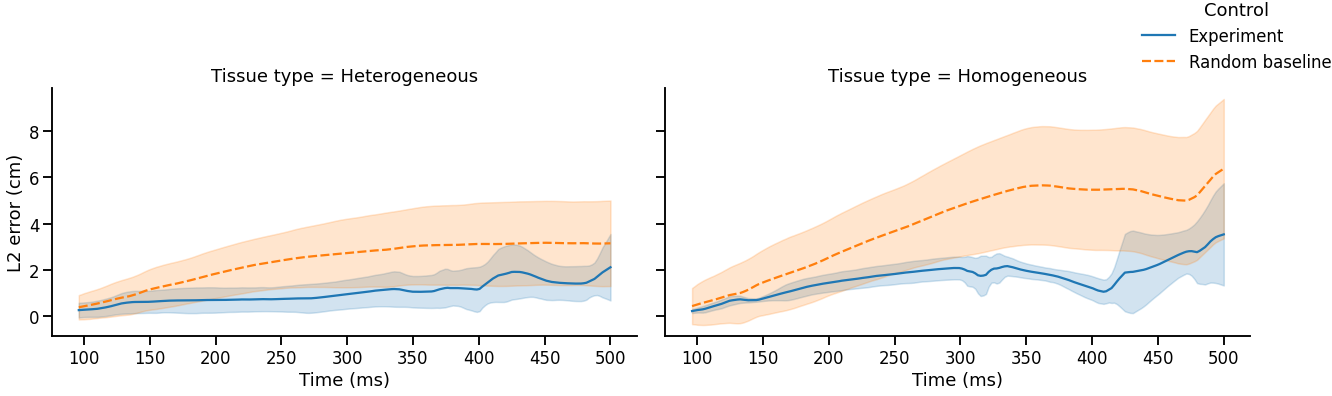
\includegraphics[width=\textwidth]{Figure-9.png}
\caption{Absolute errors between the rotor trajectories from numerically simulated and predicted data, aggregated across multiple simulations. When aggregating across trajectories we interpolate all of them along a common time vector. The shaded areas are the standard deviation. %$95$\% confidence interval of the mean.
}
\label{fig:9}
\end{figure}

\begin{figure}[!htp]
\centering
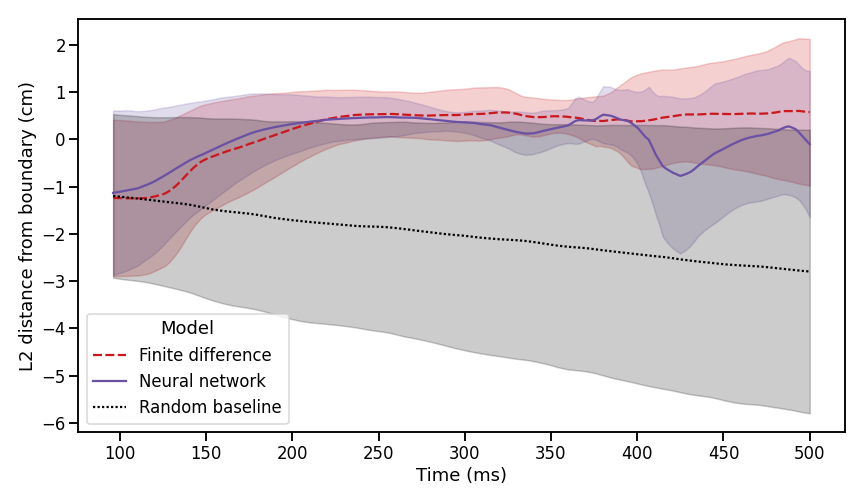
\includegraphics[width=.8\textwidth]{Figure-10.png}
\caption{Distance of rotor trajectories from the scar boundary at each point in time, aggregated across multiple simulations, for numerically simulated data (red), neural network predictions (purple) and the random baseline (black). This distance is assigned a positive value when the rotor is inside the scar, and negative when it is outside. The lines and the shaded area represent, respectively, the mean and the standard deviation across simulations.
}
\label{fig:10}
\end{figure}

% single instance
Figure~\ref{fig:8} shows two instances of trajectories of rotors, representative of (a) convergent trajectories, and (b) divergent trajectories, but converging to the boundaries of the scar. While the trajectories in Figure~\ref{fig:8}a track each other closely, the ones in Figure~\ref{fig:8}b seem to diverge after some time and converge to different sections of the scar boundary.


\subsection{Action potential dynamics}
\label{sec:results:maps}
In this experiment we assessed the properties of the action potential propagation according the activation map described in \ref{sec:methods:evaluation:maps}.
To assess how \textit{DeepX} captures these electrophysiological features already expressed by \textit{CardiAX}, figure~\ref{fig:11}a shows the normalised L$2$ errors for each activation map, averaged across 20 simulations. The normalisation, computed as the average L$2$ errors divided by the average L$2$ norm of the corresponding maps, accounts for maps that span different ranges.
To mitigate discretisation errors, each map was lightly smoothed with a $2$D Gaussian filter with standard deviation of $2$ pixels.
To account for the system chaoticity, we perform the analyses in settings that both show spiral waves and front break-ups, and simpler linear waves.
We observe that, while the errors for APA, APD, AT and the absolute CV are small, the largest error is in the RMP map, with smaller deviations observed for all the other quantities, especially the APA and the AT maps.
%\textcolor{red}{This might be due to the fact that} [\textcolor{red}{NEED INPUT TO FILL THIS GAP.}]
RMSEs are consistent for homogeneous and heterogeneous settings, showing that the \textit{DeepX} generalises to homogeneous tissue, and apply to both spiral and linear regimes, suggesting that the network performs comparably in both complex dynamics are simpler dynamics.

\begin{figure}[!htp]
\centering
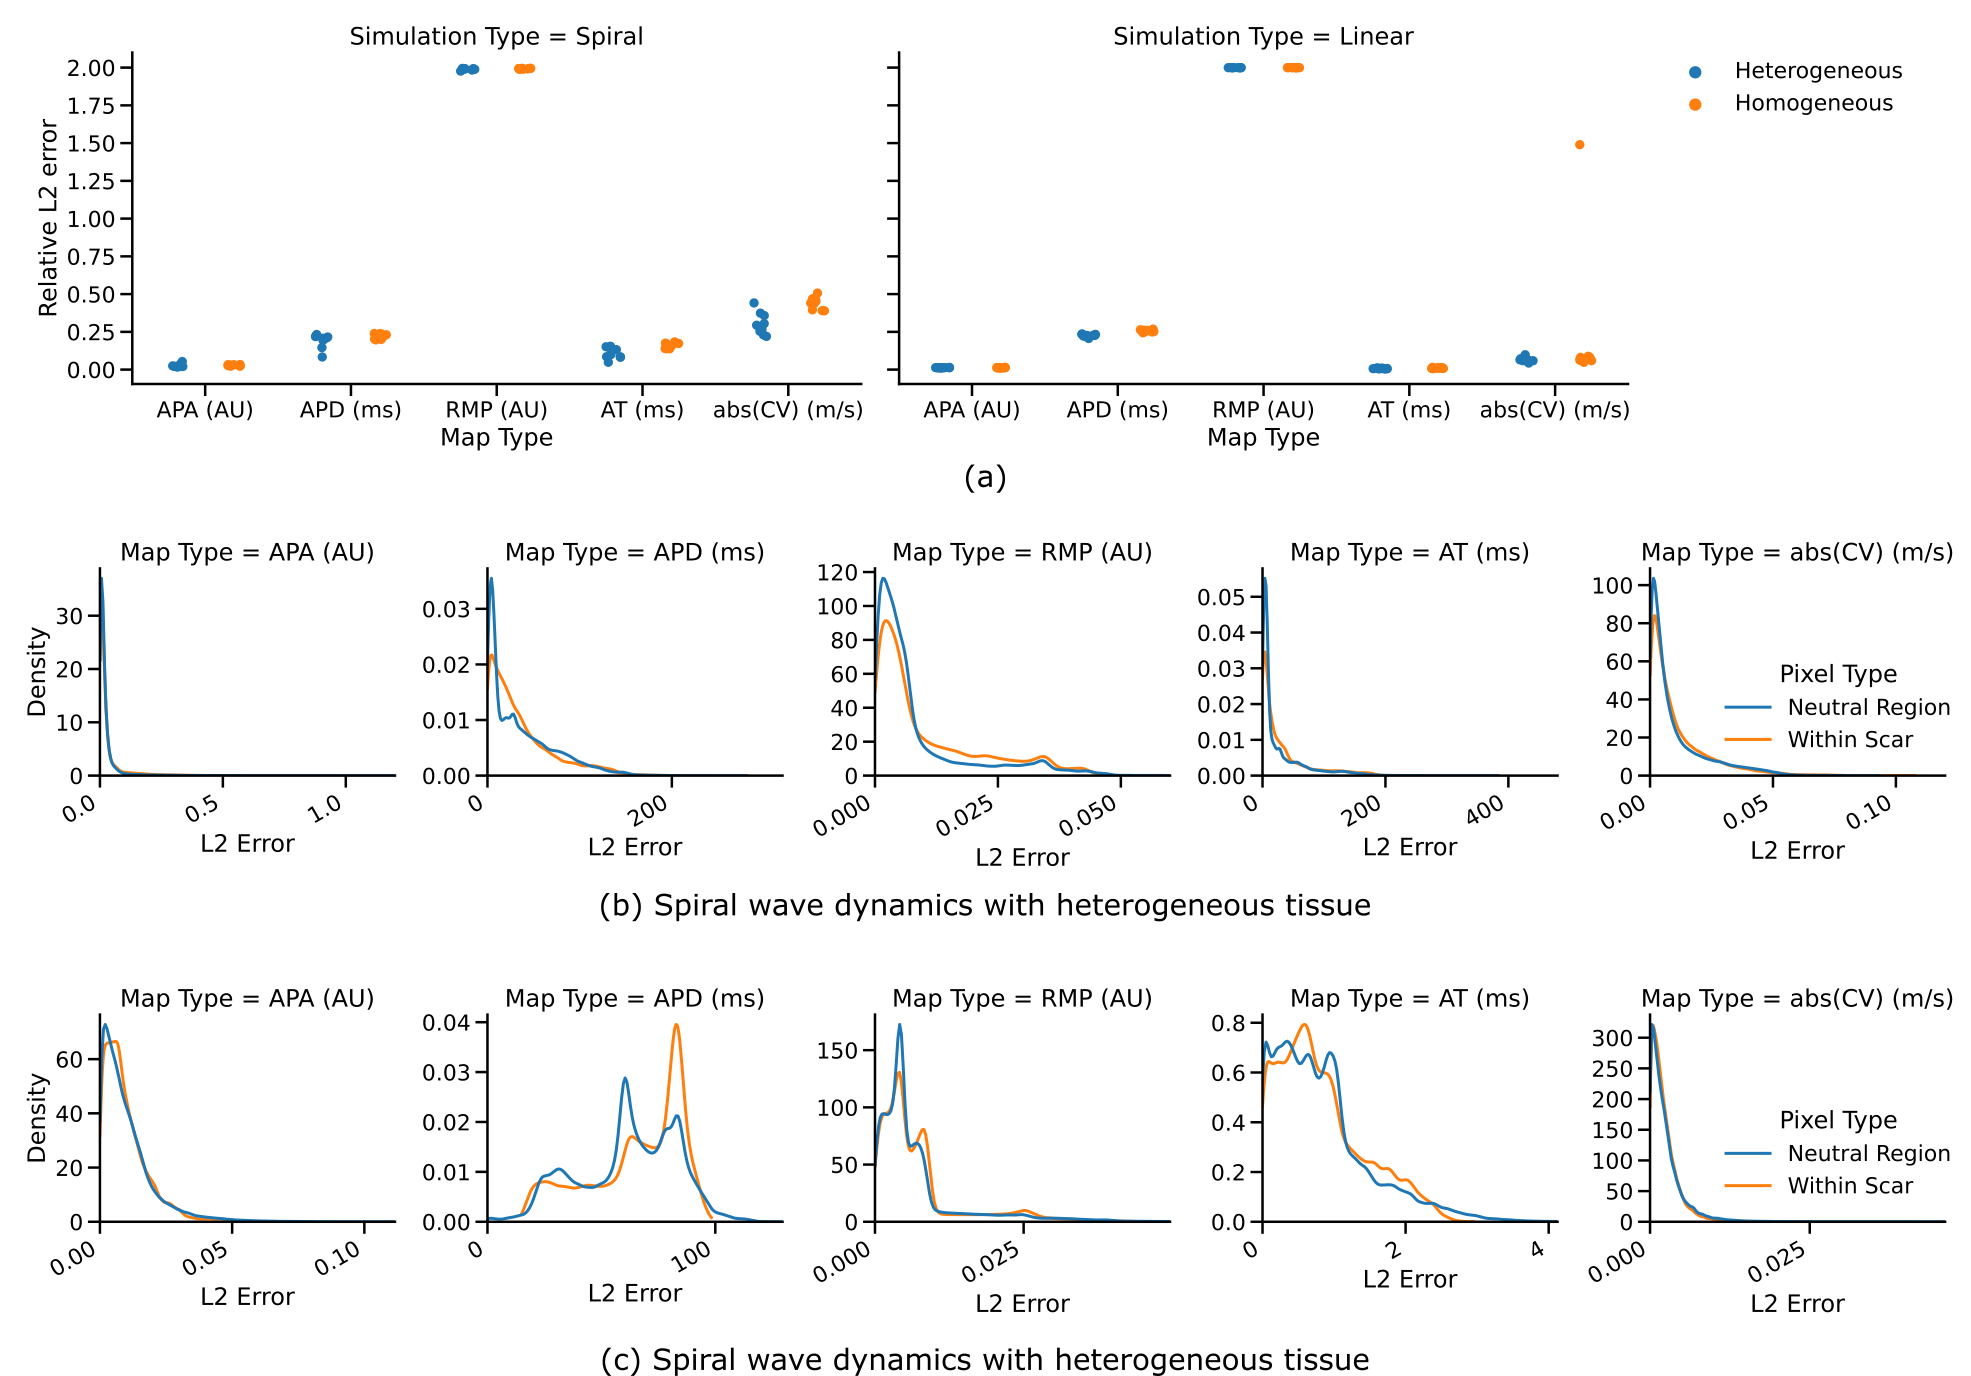
\includegraphics[width=.9\textwidth]{Figure-11.png}
\caption{(a) Comparison of average L$2$ errors for each map across multiple simulations, scaled by the average L$2$ norm of the numerically simulated and machine learnt maps. (b-c) Distribution of spatial errors between numerically simulated and machine learnt activation maps, segmented according to the type of underlying tissue (i.e. fibrotic or healthy). Results are shown for spiral (b) and linear (c) wave dynamics.
}
\label{fig:11}
\end{figure}

Figure~\ref{fig:12} shows the activation maps for a sample sequence. The first column shows the results of a \textit{CardiAX} simulation, while the second column the ones of the correspondent \textit{DeepX}. The third column displays the spatial distribution of the pixel-wise L$2$ error between the two.
While there are some apparent differences between the two models, and the maps seem susceptible to small artefacts in the predictions, there are also some common patterns.
In particular, we observe how the location of the inhomogeneity is discernible from the CV map, showing lower velocities. This was visually confirmed to be the case in most of the heterogeneous simulations analysed.

\begin{figure}[!htp]
\centering
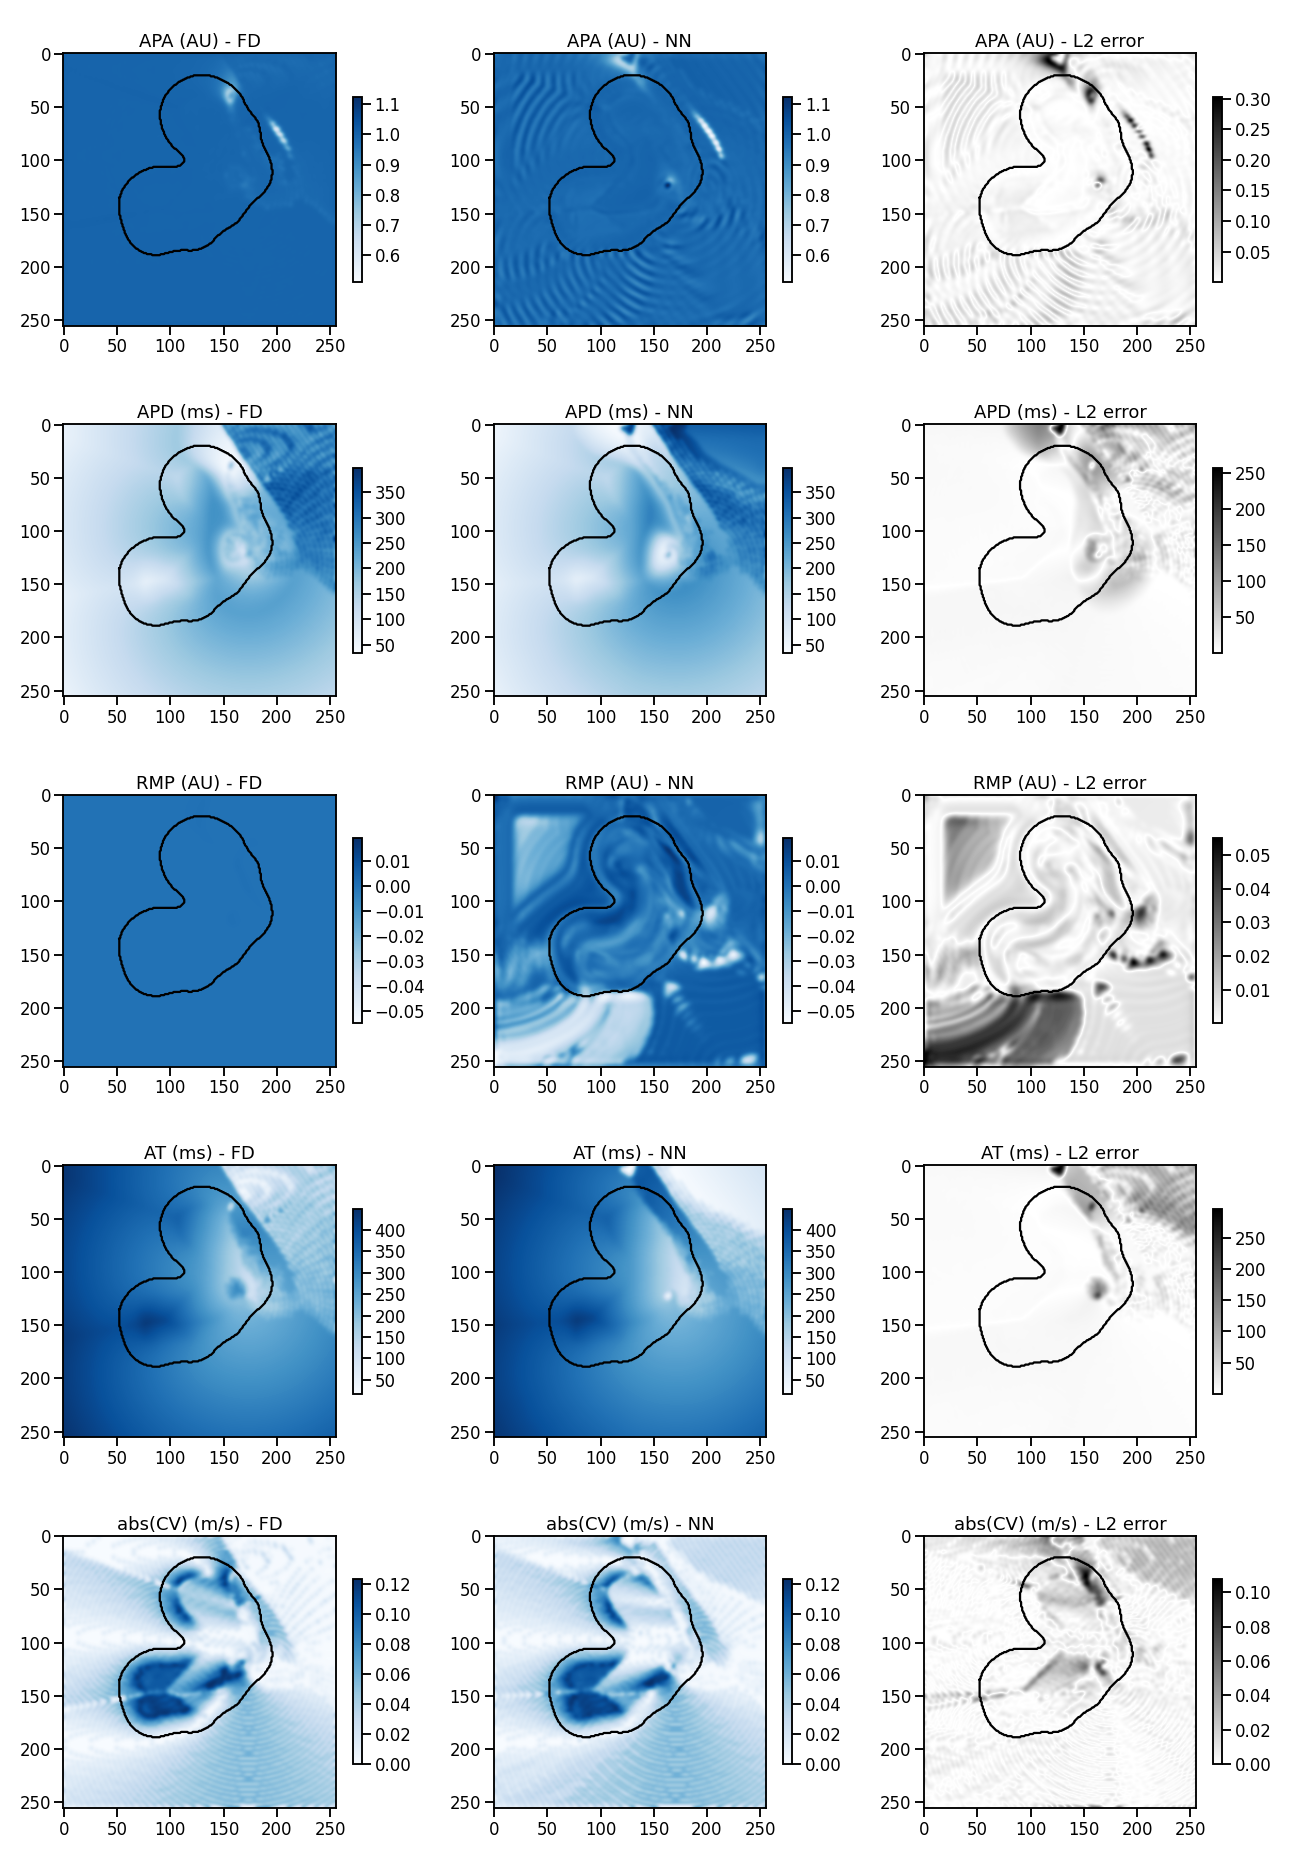
\includegraphics[width=.85\textwidth]{Figure-12.png}
\caption{Activation maps for a sample sequence, as obtained using both numerically simulated and machine learnt cardiac activity, together with the pixel-wise L$2$ error between the two.
}
\label{fig:12}
\end{figure}

Finally, to assess whether the source of the error is in the fibrotic region of tissue, we segmented the spatial errors from the activation maps according to whether they occurred inside or outside the scar boundaries. These analyses are performed on the whole set of 19 maps and results are shown in figure~\ref{fig:11}b and c, for spiral (b) and linear (c) wave dynamics. 
While the distributions are not statistically equivalent (two-sided Kolmogorov-Smirnov tests with Bonferroni correction, all p-values$<0.001$), we did not find consistent differences, in either direction, in the magnitude of errors across the different regions of the domain. That is, neither of the two error distributions was consistently stochastically greater or less than the other one, with only one exception. One-sided Kolmogorov-Smirnov tests with Bonferroni correction, returned all p-values were lower than $0.001$, aside from one of them being $0.11$. Specifically, the errors between RMP maps in the case of spiral wave dynamics tended to be greater within the inhomogeneity. 
%Indeed, all the one-sided Kolmogorov-Smirnov test with Bonferroni correction returned p-values$<0.001$, apart from the one testing the null hypothesis of ``Within Scar'' error distribution for the RMP map being stochastically greater than the ``Within Scar'' error distribution for the same map, which returned a p-value of $0.11$.
Overall, these results suggest that the neural network is able to reproduce dynamics within healthy and fibrotic tissue with comparable accuracy.


\subsection{Generalisation to different tissue sizes}
\label{sec:results:tissue_size}
Despite its translation invariance, there is no mathematical constraint that guarantees scale invariance of a CNN, i.e. that convolving the same kernel on a bigger or smaller input returns scale-invariant features, such as a spatial derivative operator.
%
In this experiment, we modulate the spatial discretisation infinitesimal $dx$ to predict the action potential dynamics on a tissue of $24cm \times 24cm$, four times the area of the tissue used during training and the same size used by \cite{Herzog2018}.
The objective of this test is to check that the spatio-temporal derivative operators learned by the neural network are invariant to the tissue size, and to understand how the network scales to higher dimensional inputs.

\begin{figure}[!htp]
\centering
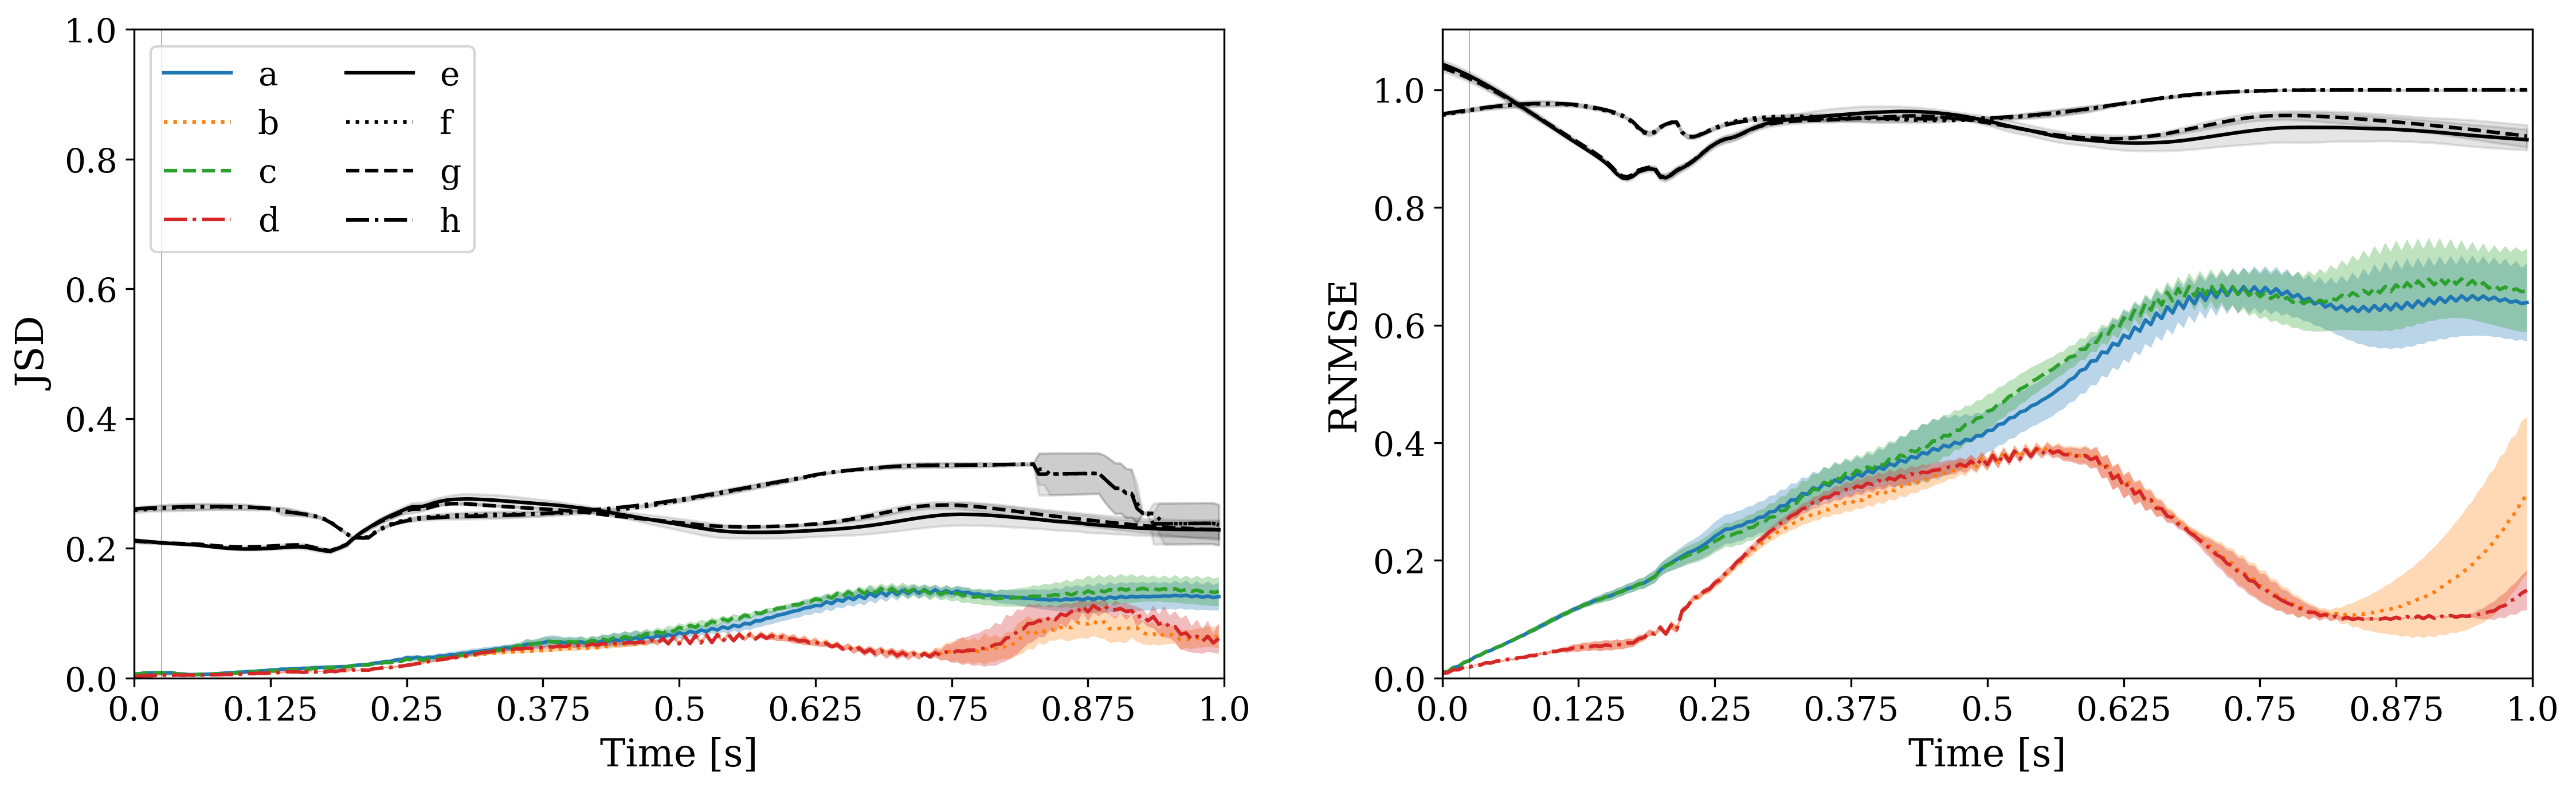
\includegraphics[width=\textwidth]{Figure-13.png}
\caption{Comparison of \textit{DeepX} and \textit{CardiAX} simulations on tissue of size $24cm \times 24cm$. Left. Jensen-Shannon divergence over time between \textit{CardiAX} simulations and its respective \textit{DeepX} one. Right. Normalised mean squared error over time between \textit{CardiAX} simulations and its respective \textit{DeepX} one.
In both plots, thick lines show the average over 10 runs randomly sampled among four conditions: either homogeneous or heterogeneous tissue, in case of linear or spiral regime. Spread area corresponds to the standard deviation over the runs. 
Black lines show control measures of JSD and RNMSE against a constant field at 0.5.
}
\label{fig:13}
\end{figure}

\begin{figure}[!htp]
\centering
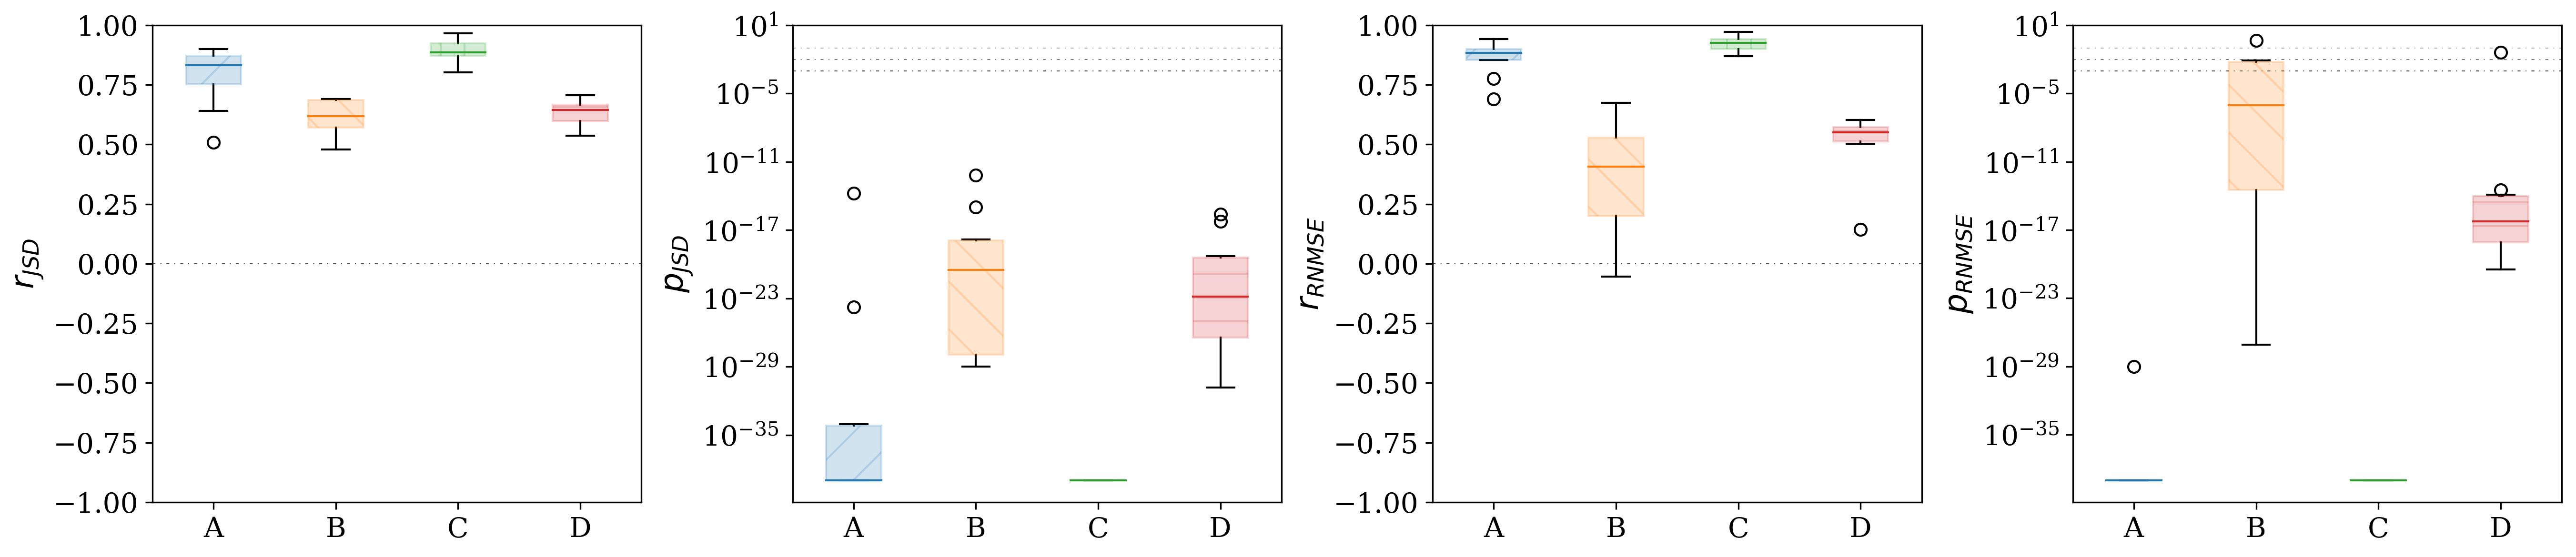
\includegraphics[width=\textwidth]{Figure-14.png}
\caption{Correlation between the errors of \textit{DeepX} simulations on tissue of size $12cm \times 12cm$ and $24cm \times 24cm$. Left. Jensen-Shannon divergence over time between \textit{CardiAX} simulations and its respective \textit{DeepX} one. Right. Normalised mean squared error over time between \textit{CardiAX} simulations and its respective \textit{DeepX} one. A. Pearson coefficient for JSD errors; B. p-values for JSD errors; C. Pearson coefficient for RNMSE errors; D. p-values for RNMSE errors.
In A and C, the grey dashed line corresponds to the a pearson coefficient of 0, no correlation. In B and D, the three shaded of black dashed lines represent threshold for $p$-values of $0.1$, $0.01$ and $0.001$, representing different levels of statistical significance.
}
\label{fig:14}
\end{figure}

Figure~\ref{fig:13} shows a comparison between the two conditions.
We observe that the error levels are consistent with the ones in \ref{sec:results:inference} for both metrics, suggesting that the model is robust to predictions on a different tissue size.
The control measure compares simulations from \textit{CardiAX} with a constant field of $0.5$.
Surprisingly, predictions on a wider tissue show reduced variance compared the predictions on $12 \times  12$ cm tissue.

To confirm the statistical relevance of these observations we measure the correlation between the errors in the two different tissue sizes using: i) the Pearson correlation coefficient ($r$) and ii) a the two-sided p-value test. 
Results are shown figure~\ref{fig:14}.
For the JSD we report a $r_{JSD} = 0.73 \pm 0.14 $ and all $p_{JSD}$-values $< 0.001$.
For the RNMSE, measures are $r_{RNMSE} = 0.66 \pm 0.27 $ and $p_{RNMSE}$-values $< 0.01$  and $p_{RNMSE}$-values $< 0.001$ in 90\% of the cases.



\section{Discussion}
\label{sec:discussion}
% chaoticity
The growth of the error in time described in \ref{sec:results:inference}, in the case of spiral waves, is consistent with the assumption of chaoticity hypothesised in \ref{sec:methods:evaluation}.
One explanation for this behaviour is that the error grows for small inaccuracies in the model, which causes the system to settles into a different orbit, while the ionic model is still consistent. 
Instead, linear waves show more stable equilibria.
The discrepancies in behaviour between spiral and linear wave regimes suggests that the network is reasonably accurate in non-chaotic scenarios, and that most of the error is caused by the divergence of the solution towards different orbits.
This is confirmed by the small errors found in the activation maps described in \ref{sec:results:maps}.

The difference between the training horizon, $25$ms (5 Euler steps), and the testing horizon ($1000$ms, 200 Euler steps) is significant. The results reported in \ref{sec:results:inference}, \ref{sec:results:electrograms} and \ref{sec:results:maps} provide evidence that, despite this difference, the model generalises well to longer sequences. Furthermore, the propagation function learned from experimental data is stable in conditions where the time integration interval is high, whilst maintaining a reasonable level of generalisation and applicability to different scenarios.
Also this scenario is compatible with the dynamical properties described in \ref{sec:methods:evaluation} and confirms the assumption.

% incorporate info about diffusivity
On an orthogonal dimension, the agreement between the errors in the heterogeneous cases and the homogeneous ones shown in \ref{sec:results:inference}, \ref{sec:results:electrograms} and \ref{sec:results:tissue_size} shows very competitive performance when the inhomogeneities are not present.
Since the network has never observed data coming from the homogeneous tissue distribution during training, the recovery of the homogeneous solution of the monodomain equation suggests that \textit{DeepX} learned to encode information about diffusivity into the spatio-temporal integration operator.
In case of overfitting we would expect the model to not respond well when no scar is present, and provide biased responses, e.g. showing localised wavefront bending in regions where there is no inhomogeneity.
The hypothesis that the network learned a code for diffusivity is also confirmed by the results in \ref{sec:results:maps}, where the fibrotic tissue is discernible from the \textit{activation maps}. 


The small errors found in the ADP~90 maps shows that \textit{DeepX} correctly captures the dynamics of depolarisation of the wavefront and incorporates a most of the ionic complexity underlying the relationship between pulse duration and tissue recovery \cite[]{Fenton1998}.
Analogously, the good approximation of the CV restitution map shows that the network can encoded the dynamics of the repolarisation of the waveback.

% oscillations in the predictions
One interesting phenomenon visible in figure~\ref{fig:3}, \ref{fig:5} and \ref{fig:13} is the presence of high frequency oscillations in the errors.
This is particularly evident when the tissue is in recovery. In particular, in figure~\ref{fig:3} we can observe that, in the case of linear waves, when the RMSE decreases, and the tissue settles back into the resting potential, the JSD starts to oscillate at this high frequencies.
This inaccuracy of the model when the tissue depolarises is congruous with the scarce  results on the RMP maps.
One hypothesis that can explain this symptom is the high variance of spatial gradients between the $w$ variable and the $u$ and $v$ variables. This difference could require the neural network to learn a very diverse set of convolutional filters to approximate such variance, making the optimisation problem more difficult.


\subsection{Limitations and future directions}
\label{sec:discussion:limitations}
% Two dimensions
Experiments are limited to the monodomain equation in two-dimensional, planar geometries. The main challenge in scaling-up to three-dimensional domains can ascribed to the curse of dimensionality: the number of possible permutations of data grows exponentially with the growth of dimensionality \cite[]{bellman1966dynamic}. Solving the curse of dimensionality is still an open problem in the wider machine learning domain.

% Ionic model
Inference is limited to the ionic model proposed by \cite{Fenton1998}, the three-currents Fenton-Karma. Using a different ionic model with a number of latent variables close to three poses no visible challenges. Scaling up to a high number of variables, such as the models in  \cite{TenTusscher2006ComparisonTissues} and 
\cite{Iyer2004AMyocyte}, could face the same dimensionality problem discussed for the geometry of the domain.

% Parameter set
The physical properties of the tissue are fixed in all experiments to the parameter set 3 described in \cite{Fenton2002}. Optimising the model using a different set of parameters is straightforward, albeit not the focus of this work. Instead, constructing a parameterised model that allows modulating these quantities, with such a high degree of freedom, is an unsolved challenge in deep learning \cite[]{kim2019deep}.

% Isotropy
The diffusivities used in the experiments present isotropic conductances. Anisotropy could be incorporated by splitting the diffusivity map $D$ in two components $D_\bot, D_\parallel$, and presenting it to the network as another dimension in the inputs.

% Stimuli
Our architecture lacks the support for presenting stimuli in the middle of a simulation, whilst keeping the state of the ionic model consistent. The current approach is to add the external current to the $u$ variable, which causes the ionic state to be inconsistent in the moments after excitation. This can be addressed by adding a fifth dimension to the inputs of the network that contains the spatial distribution of the external current at the specific time $t$.

% clinical relevance
All the experiments are carried using \textit{in-silico} data. Collecting action potential data from \textit{in-vivo} experiments could help gain a better understanding of the error distribution of current rule-based models.
The inability to clinically observe fictitious latent variables from functioning cardiac tissue requires discovering ionic models from data.
By constraining the network only on the action potential, the main challenge here is to achieve good fitting while formulating the problem as Markovian with respect to the action potential alone.

% optimisation
The optimisation process suffers from high variance around extrema.
The use of additional loss functions to capture physiologically relevant properties of the target distribution is a potential sources of improvement.
One example is the use of loss functions that act in a non observable space \cite[]{johnson2016perceptual}, such as the ones employed in image synthesis and video processing \cite[]{zhang2018unreasonable,lai2018learning}. Constraining the optimisation problem in the space of the activation maps and the electrograms described in \ref{sec:methods:evaluation:maps} and \ref{sec:methods:evaluation:electrograms} could help smoothing the loss function and avoid plateaus.


\section{Related work}
\label{sec:related_work}
In modelling electrophysiology of the heart, \cite{Herzog2018} combined a convolutional neural network with a linear chain of conditional random fields to learn the dynamics of the \cite{Bueno-Orovio2008MinimalTissue} model.
Unlike previous research, this method scales up to very high dimension data.
\cite{Cantwell2019RethinkingModelling} proposed an encoder-decoder structure to predict two-dimensional diffusion in heterogeneous media. The model uses convolutions and transposed convolutions interleaved with batch normalisation \cite[]{Ioffe2015BatchShift} and ReLU non-linearities to compress the AP observations into a latent representation.
Between the encoder and the decoder is a convolutional LSTM \cite[]{Shi2015ConvolutionalNowcasting, Hochreiter1997LongMemory, Zaremba2014RecurrentRegularization} that acts as an integrator in time.
The reuse of the weights of the LSTM vaguely resembles the structure of weight-tied neural networks proposed for natural language processing \cite[]{Press2017UsingModels, Inan2017TyingModeling}, and later extended to two-dimensional sequences \cite[]{bai2018trellis}.

% reaction-diffusion
Cross fertilisation between the research on PDEs and studies on computer vision catalysed the research on deep learning to learn formulations of the wave equation from data.
\cite{Li2020ReactionNetwork} proposed to predict the evolution of spatial density resulting from the Zeldovich equations, a reaction diffusion equation used to simulate combustion. A U-net architecture maps the density state at the current time, and the target time variable, the objective density state. Their results show that the application is limited to low dimensional data.
\cite{Stanziola2020AUltrasound} proposes to solve the lossless Helmholtz equation with heterogeneities in the speed of sound map, by learning an iterative optimiser.
\cite{Bar-Sinai2019LearningEquations} proposed to reduce the computational costs of solving a PDE by using proxy spatial gradients defined on a coarser grid. Despite the improved accuracy, this data-driven discretisation is computationally more expensive than canonical rule-based discretisations, which limits its applicability to very low dimensional problems.
Finally, \cite{Kelly2020LearningSolve} explores the benefits of regularising the learning routine by minimising derivatives of the order of the PDE of interest. \cite{Raissi2019Physics-informedEquations} uses neural networks as implicit neural representations of single solutions to forward and inverse problems by including a specific loss term that forces the solutions to obey known physical laws. This approach was employed by \cite{SahliCostabal2020Physics-InformedMapping} to solve the eikonal equation in the left atrium and estimate high-resolution activation time maps.


%%  SUMMARY AND CONCLUSION
\section{Conclusions}
\label{sec:conclusions}
The computational modelling of cardiac electrical activity plays an important role
to improve decision making on the treatment of heart rhythm disorders.
The primary purpose of this study is to bring the science closer to rapid patient-specific modelling.
We focus on a class of reaction-diffusion equations that are widely used for studying macroscopic-scale electrical behaviour in cardiac tissue and can capture a broad spectrum of action potential propagation dynamics.
We explore the benefits of deep learning to augment numerical modelling in tissue with localised inhomogeneities by proposing a recurrent convolutional residual network, \textit{DeepX}. The model is optimised to learn the solution to the monodomain equation coupled with the Fenton-Karma \cite[]{Fenton1998} ionic model in two-dimensional geometries.
While completed research on the topic investigated the problem of low-dimensional data, we provide, to the best of our knowledge, the first application on high dimensional data with heterogeneities.
Under canonical evaluation metrics, solutions are most accurate when the system has a stable equilibrium. In complex re-entrant regimes that give rise to chaotic dynamics and multiple orbits, \textit{DeepX} qualitatively captures important features of the cardiac model, such as the pinning of reentrant waves to the boundary of inhomogeneities, the action potential duration, action potential activation, activation time, conduction velocities, and electrograms. Overall, the model can encode information about diffusivity.

In short, the paper provides the following outputs:
\begin{itemize}
\item \textit{CardiAX}, a fast end-to-end, differentiable, finite difference solver with GPU acceleration.
The main function of the solver is to enable fast incremental development through quick iterations between data-generation and network optimisation cycles.
\item \textit{FKset}, a publicly available dataset containing spatio-temporal sequences generated using the Fenton-Karma equations.
\item \textit{DeepX}, a deep residual convolutional network composed recursively to integrate in time, used to approximate the solution to the Fenton-Karma equations in tissue with heterogeneities.
\end{itemize}

Our model captures important features of the dynamical system, showing that data-driven techniques are favourable candidates to solve the forward problem of predicting the evolution of electrical activation for patient-specific treatments.

\section*{Conflict of Interest Statement}
%All financial, commercial or other relationships that might be perceived by the academic community as representing a potential conflict of interest must be disclosed. If no such relationship exists, authors will be asked to confirm the following statement: 
The authors declare that the research was conducted in the absence of any commercial or financial relationships that could be construed as a potential conflict of interest.

\section*{Author Contributions}
C.D.C and A.A.B. conceived the idea, supervised the work, wrote and edited the manuscript.
E.P. developed the methodology, implemented the software, generated and curated the data, designed and trained the model, performed the experiments, wrote and edited the manuscript, and prepared the related graphics.
S.G. implemented the code for scar generation, performed the experiments, analysed the results, prepared the related graphics and wrote and edited the manuscript.
M.V. analysed the results, edited the manuscript and provided a critical review. S.F., M.L. and N.S.P edited the manuscript and provided a critical review.

\section*{Funding}
E.P., C.D.C, A.A.B, S.G and N.S.P are funded by the Rosetrees Trust grant n.M577.
S.F is funded by a scholarship from Imperial's Department of Biongineering. M.L is funded by a scholarship from Imperial's Department of Aeronautics. 
Open access fees are provided by the Imperial College London Open Access Fund.

% \section*{Acknowledgments}
% \section*{Supplemental Data}
%  \href{http://home.frontiersin.org/about/author-guidelines#SupplementaryMaterial}{Supplementary Material} should be uploaded separately on submission, if there are Supplementary Figures, please include the caption in the same file as the figure. LaTeX Supplementary Material templates can be found in the Frontiers LaTeX folder.

\section*{Data Availability Statement}
The datasets generated for this study and the relative codebase can be found in this repository on GitHub, at https://github.com/epignatelli/cardiax.
The source code for both the CardiAX solver and the neural network solver is accessible at \hyperlink{https://github.com/epignatelli/cardiax}{https://github.com/epignatelli/cardiax} for non-commercial use only.
The data used in the experiments is available at https://bit.ly/37BabEm.
\Edu{Anil, Chris, do you think we can have a box place to save the data permanently?}

\bibliographystyle{frontiersinSCNS_ENG_HUMS} % for Science, Engineering and Humanities and Social Sciences articles, for Humanities and Social Sciences articles please include page numbers in the in-text citations
% \bibliographystyle{frontiersinHLTH&FPHY} % for Health, Physics and Mathematics articles
\bibliography{references}

\end{document}
